\documentclass[a5paper,pagesize,DIV=14]{scrbook}

\usepackage[french]{babel}
\usepackage[utf8]{inputenc}
\usepackage[T1]{fontenc}
\usepackage{graphicx}
\usepackage{tabularx}
\usepackage{color}
\usepackage{tikz}
\usepackage{url}
\usepackage{chessboard}
\usepackage{import}
\usepackage{pdfpages,wrapfig}

\setlength{\parskip}{\smallskipamount}
\setlength{\parindent}{0pt}

%%\newcommand{\maisonPair}[5]{ \begin{tikzpicture}
  \node[name=m,shape=regular polygon,regular polygon sides=#3,minimum size=22mm,rotate=(360/#3)]{};
  \node[name=b,shape=regular polygon,regular polygon sides=#4,minimum size=14mm,rotate=(360/#4)/2]{};
  \foreach \base/\maison in {#5} {
    \draw[shift=(m.corner \base)]
       node[shape=ellipse,fill=\maison,draw=black,rotate=((360/#3)*(\base-1))+(360/#3/2)] {~~};
  }
  \foreach \bb in {1,...,#4} {
    \draw[shift=(b.corner \bb)] node[name=bb \bb]{};
  }
  \foreach \base/\maison in {#1} {
    \draw[shift=(b.corner \base)]
       node[name=bb \base,shape=circle,fill=\maison,draw=black,inner sep=.1]
       {~~~};
%         {\footnotesize\base};
  }
  #2
\end{tikzpicture} }
\newcommand{\maisonImpair}[5]{ \begin{tikzpicture}
  \node[name=m,shape=regular polygon,regular polygon sides=#3,
        minimum size=22mm, inner sep=0pt]{};
  \node[name=b,shape=regular polygon,regular polygon sides=#4,minimum size=14mm]{};
  \foreach \base/\maison in {#5} {
    \draw[shift=(m.corner \base)]
       node[shape=ellipse,fill=\maison,draw=black,rotate=(360/#3)*(\base-1)] {~~};
  }
  \foreach \base/\maison in {#1} {
    \draw[shift=(b.corner \base)]
       node[shape=circle,fill=\maison,draw=black,inner sep=.1] {~~~};
  }
  \foreach \bb in {1,...,#4} {\draw[shift=(b.corner \bb)] node[name=bb \bb] {};}
%  \foreach \bb in {1,...,#4} {\draw[shift=(b.corner \bb)] node[name=bb \bb]{\tiny\bb};}%debug the bonshommes names
  #2
\end{tikzpicture} }

\newcommand{\maisonQuatre}[2]{\maisonPair{#1}{#2}{4}{12}{1/A,2/B,3/C,4/D}}
\newcommand{\maisonCinq}[2]{\maisonImpair{#1}{#2}{5}{20}{1/A,2/B,3/C,4/D,5/E}}
\newcommand{\maisonSix}[2]{\maisonPair{#1}{#2}{6}{24}{1/A,2/B,3/C,4/D,5/E,6/F}}
\newcommand{\maisonSept}[2]{\maisonImpair{#1}{#2}{7}{28}{1/A,2/B,3/C,4/D,5/E,6/F,7/G}}

\colorlet{A}{green!60}
\colorlet{B}{red!80}
\colorlet{C}{purple!40}
\colorlet{D}{black!2!yellow}
\colorlet{E}{blue!70}
\colorlet{F}{orange!80}
\colorlet{G}{olive}
\colorlet{H}{magenta}
\colorlet{I}{lime}
\colorlet{J}{pink}

\newcommand{\pawn}[1]{\tikz \draw node[shape=circle,fill=#1,draw=black,inner sep=.1] {~~~};}



%%%%%%%%%%%%%%%%%%%%%%%%%%%%%%%%%%%%%%%%%%%%%%%%%%%%%%%%%%%%%%%%%%%%%%%%%%%%%%%%%%%%%%%
\begin{frame}{Activité: Base-ball multicolore}
  \begin{block}{Matériel nécessaire}
    \begin{itemize}
    \item Plusieurs équipes bien différentiables, chacune composée d'une maison et de deux bonshommes (des legos, des bouts de bois, des cailloux, du fil électrique de différentes couleurs, ou autres) 
    \item 4 équipes au minimum. On peut mettre des équipes supplémentaires pour augmenter la difficulté.
    \end{itemize}
  \end{block}

  \begin{block}{Règles du jeu (exemple à quatre équipes)}
    \begin{itemize}
      \item \structure{Installation :} disposer 4 maisons autour du terrain et répartir 7 bonshommes au hasard sur les maisons (le bonhomme restant n'est pas utilisé).
      \item \structure{Coup autorisé :} déplacer un seul bonhomme à la fois, vers la maison contenant un seul bonhomme, depuis une des deux maisons voisines (interdit de traverser le terrain).
    \item  \structure{Objectif :} Ramener tous les bonshommes dans la maison de leur couleur.
    \end{itemize}
  \end{block}

  \bigskip

  \begin{columns}
    \begin{column}{0.27\linewidth}
    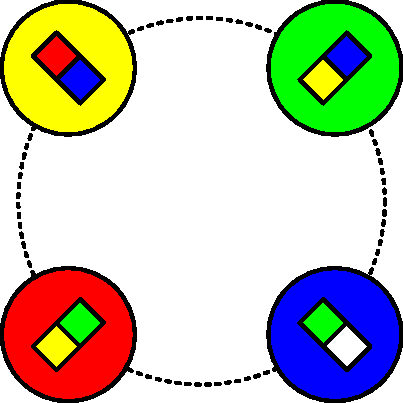
\includegraphics[width=\linewidth]{img/baseball_init.pdf}\\
    \center{État initial}
    \end{column}
    \begin{column}{0.27\linewidth}
    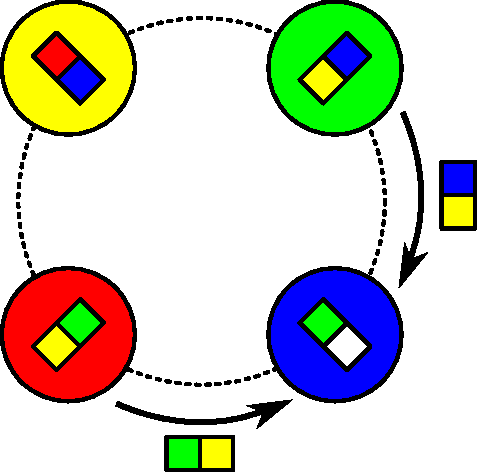
\includegraphics[width=\linewidth]{img/baseball_coup.pdf}\\
    \center{Coup autorisé}
    \end{column}
    \begin{column}{0.27\linewidth}
    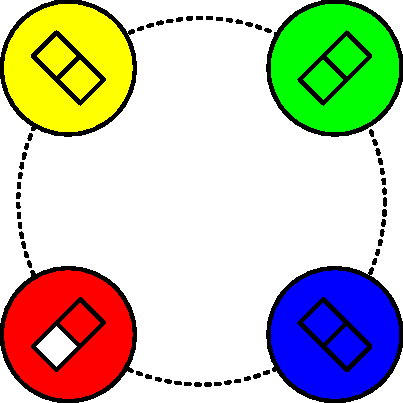
\includegraphics[width=\linewidth]{img/baseball_final.pdf}\\
    \center{État final}
    \end{column}
  \end{columns}

  \bigskip
  \begin{block}{Objectif de l'activité}
    Le plus important dans cet exercice n'est pas tant de résoudre le problème que d'\structure{expliquer clairement} comment on fait. On cherche donc l'\alert{algorithme} permettant de résoudre le problème.
  \end{block}
\end{frame}
%%%%%%%%%%%%%%%%%%%%%%%%%%%%%%%%%%%%%%%%%%%%%%%%%%%%%%%%%%%%%%%%%%%%%%%%%%%%%%%%%%%%%%%%%
%\newcommand{\flecherond}[1]{
  %\draw[ultra thick] (0,0) circle (3mm);
  %\draw[ultra thick,rotate=#1*72] (3mm,0) -- +(-.15,-.08);
  %\draw[ultra thick,rotate=#1*72] (3mm,0) -- +(.08,-.15);
  %\draw[fill=white,draw=white,rotate=#1*72] (3mm,2.5pt) circle (2pt);
%}
\begin{frame}{Un premier algorithme pour le base-ball multicolore}
  En suivant les règles du jeu, on observe que quelque soit la disposition des bonshommes, il existe toujours 4 coups possibles : déplacer vers la case vide un des 4 bonshommes présents dans les deux maisons voisines.

  Notre algorithme sera donc une méthode permettant de choisir à chaque étape quel coup jouer parmis les 4 possibles.

  \begin{block}{L'algorithme}
    \begin{itemize}
    \item On ne s'autorise à tourner que dans un seul sens. Ainsi, le nombre de coups possibles descends de 4 à 2 (car 2 bonshommes tourneraient à l'envers).
    \item Parmis les 2 coups restants, on déplace le bonhomme qui a la plus grande distance à parcourir avant d'arriver à sa maison (Si la distance est la même, c'est que les deux bonhommes ont la même couleur - les deux coups sont donc équivalents).
    \end{itemize}
  \end{block}

  \begin{block}{Exemple d'exécution}
    \begin{center}
      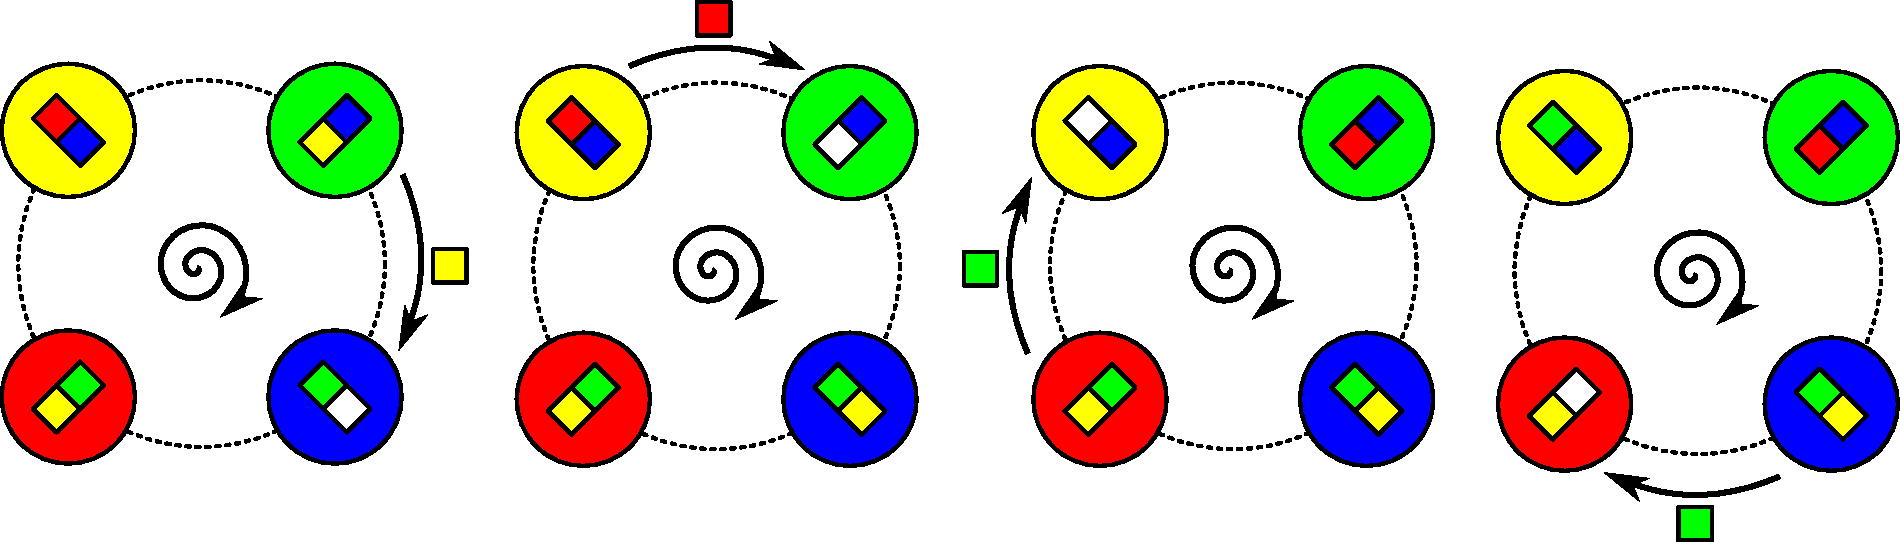
\includegraphics[width=\linewidth]{img/baseball_ex1.pdf}
    \end{center}

  Ici, nous n'avons représenté que les 4 premières étapes. mais l'algorithme arrive à la solution en 15 étapes.
  \end{block}
\end{frame}

\begin{frame}{Étude du premier algorithme pour le base-ball multicolore}
  \begin{block}{Cet algorithme semble attirant}
    \begin{itemize}
    \item Il est très simple: on pourrait l'expliquer à un ordinateur
    \item Il est relativement rapide: 15 coups pour 7 bonshommes, ce n'est pas si mal
    \item Seul problème: cet algorithme est faux: dans certains cas, il ne termine jamais\ldots
    \end{itemize}
  \end{block}

  \begin{block}{Exemple d'exécution incorrecte}
    Il suffit de partir d'une situation gagnée et d'inverser deux bonshommes pour mettre notre algorithme en échec.
\end{block}
  \begin{center}
    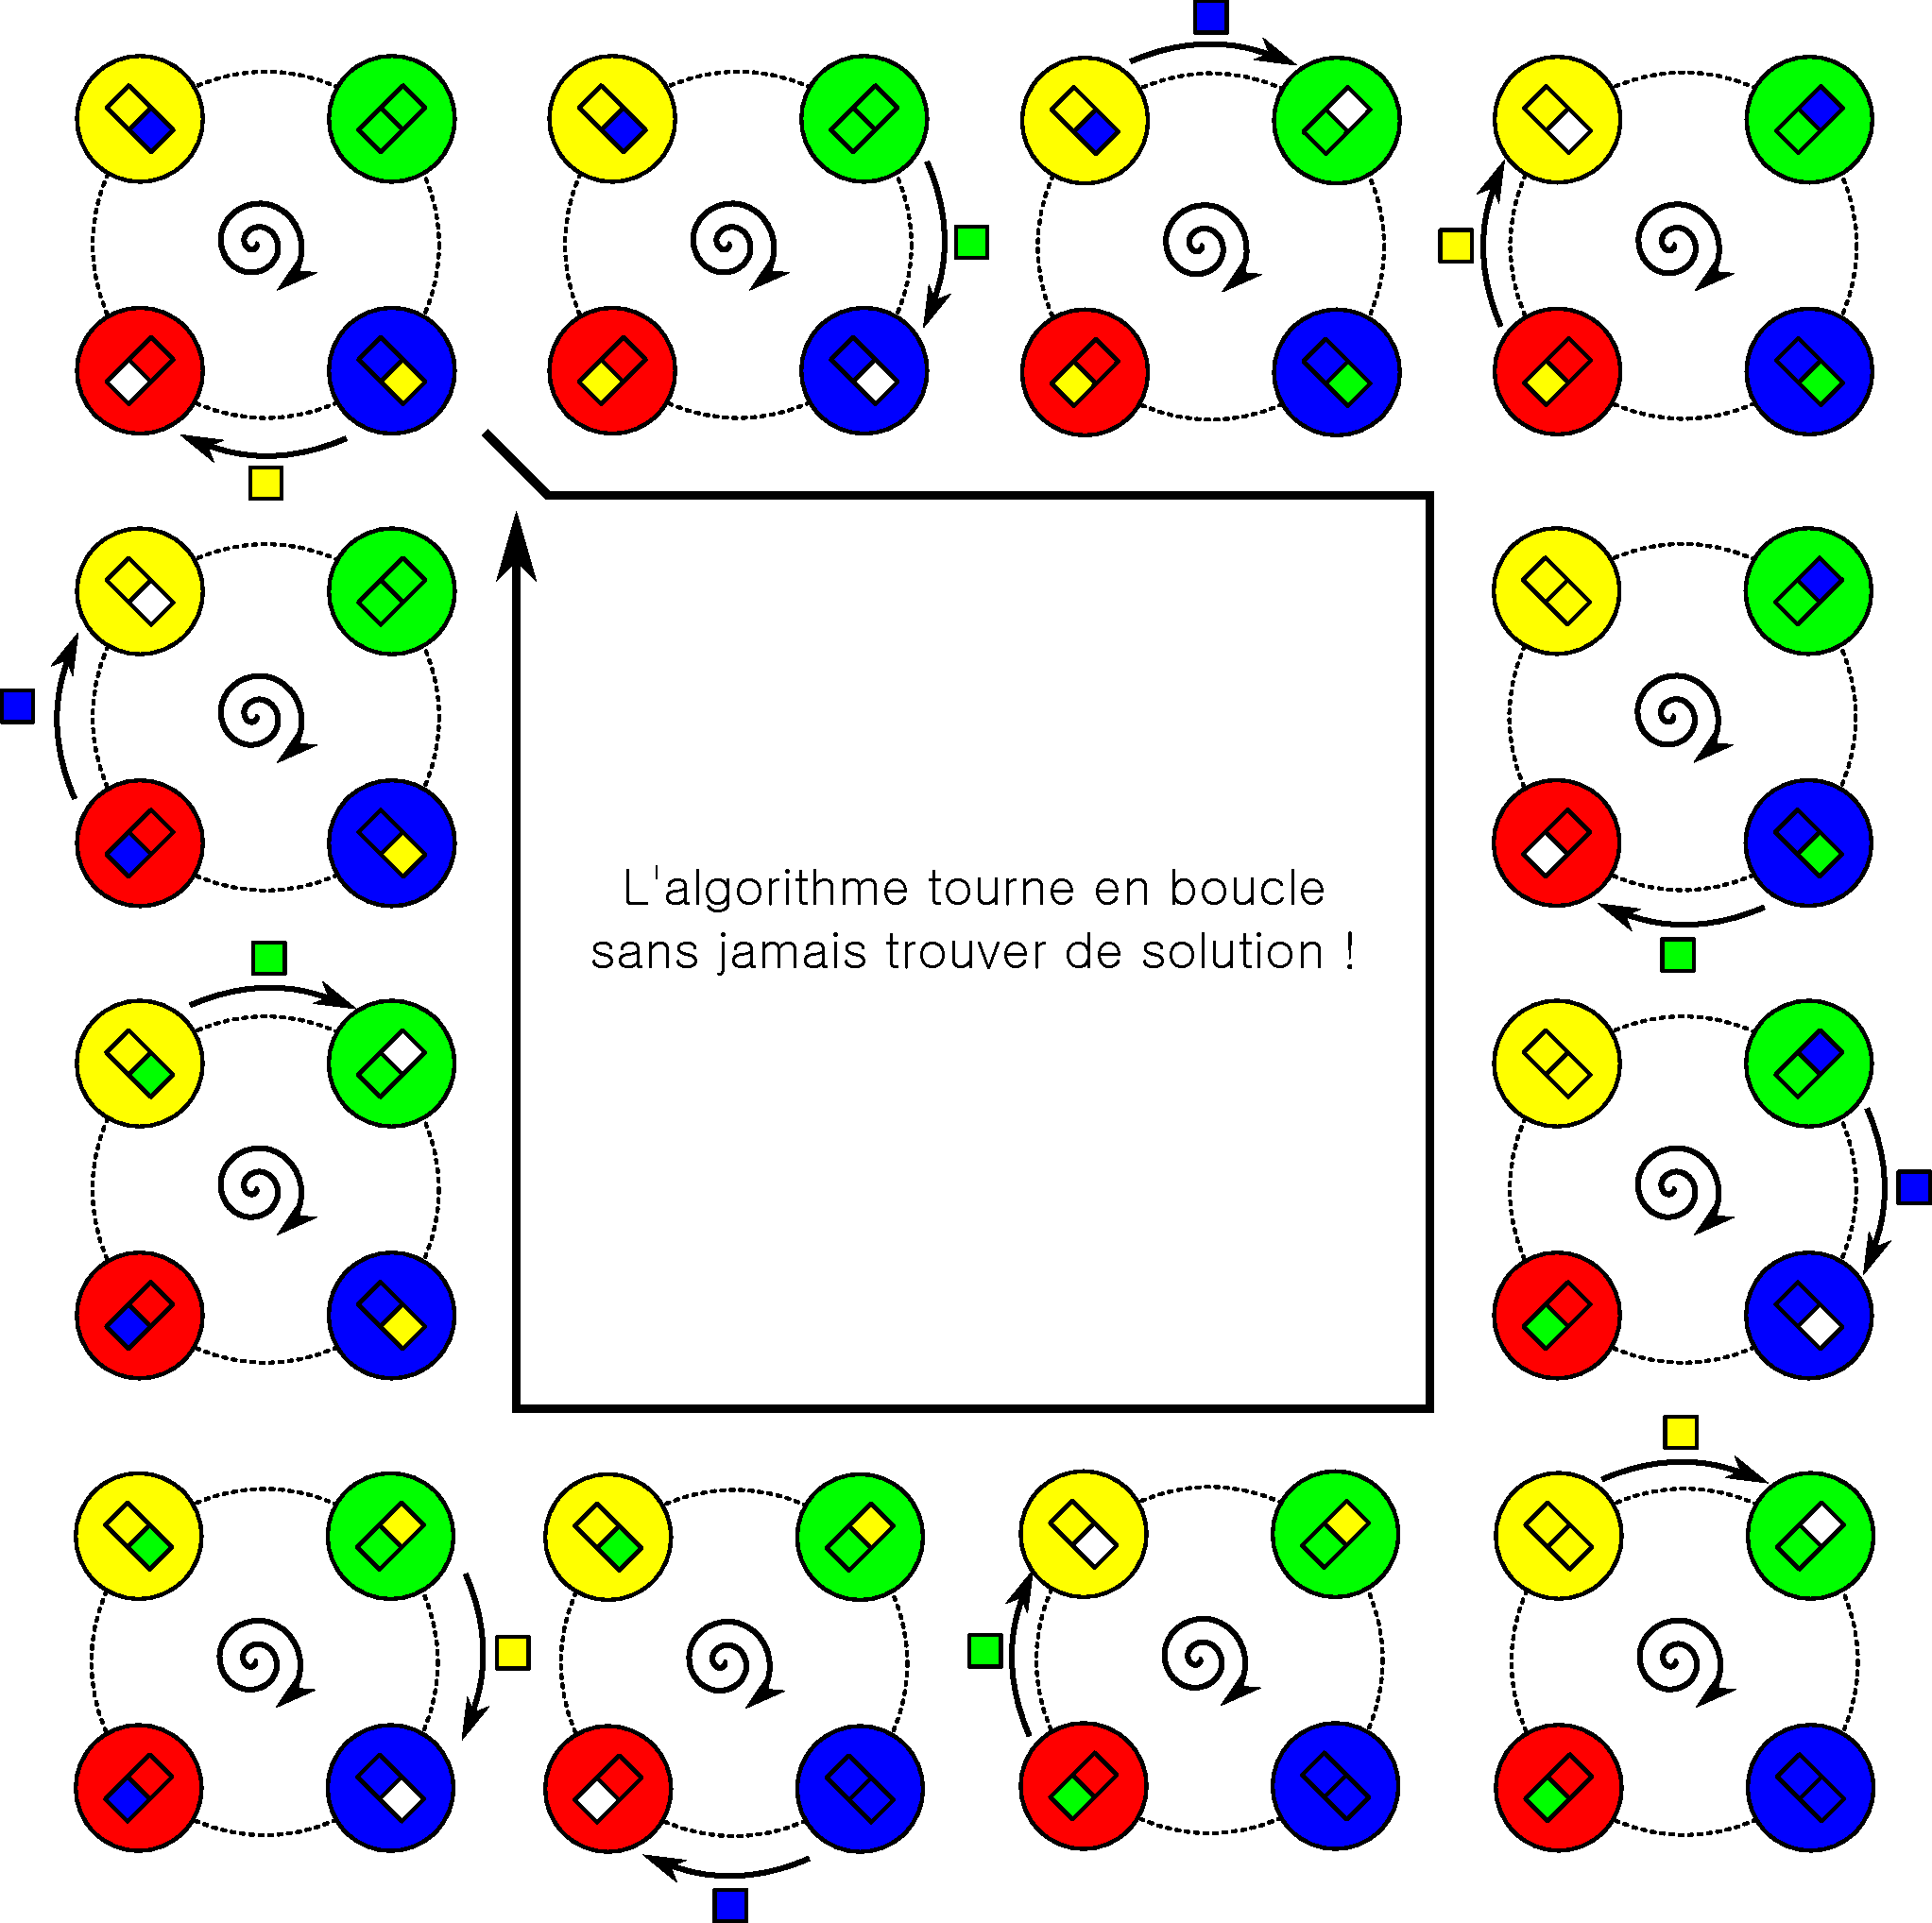
\includegraphics[width=0.8\linewidth]{img/baseball_ex2.pdf}
  \end{center}
\end{frame}

%%%%%%%%%%%%%%%%%%%%%%%%%%%%%%%%%%%%%%%%%%%%%%%%%%%%%%%%%%%%%%%%%%%%%%%%%%%%%%%%%%%%%%%%
\begin{frame}{Un autre algorithme pour le base-ball multicolore}
  \begin{block}{Apprendre de ses échecs: {\color{black}notre algorithme boucle parfois à l'infini}}
    \begin{itemize}
    \item Pour réparer cela, le plus simple est de s'interdire de boucler, en
      coupant le cercle.
    \item Pour ne pas se tromper, le plus simple est de placer les maisons en ligne.
    \end{itemize}

    \begin{center}
      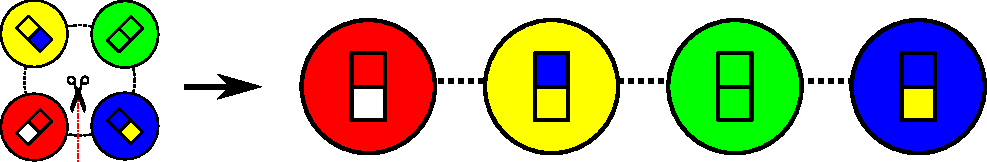
\includegraphics[width=0.8\linewidth]{img/baseball_ligne.pdf}
    \end{center}
  \end{block}

  \bigskip

  \begin{block}{Apprendre de ses réussites: {\color{black}le crépier}}
    \begin{itemize}
    \item On a cherché à réduire la taille du problème à peu à peu\\
      {(il y a 7 crèpes à trier. La plus grande va définitivement à sa place; il
        reste 6 crèpes à trier)}
    \item On s'est fixé des objectifs intermédiaires, qui décomposent le
      problème en étapes que je sais faire\\
      {(mettre la plus grande en haut pour parvenir à la mettre en bas)}
    \end{itemize}
  \end{block}

  \begin{block}{Nouvel algorithme}
    \begin{itemize}
    \item On s'occupe d'abord des bonshommes de la première maison, et on n'y touche plus ensuite.
    \item On répète pour la deuxième maison, et ainsi de suite pour toutes les autres.
    \item Pour ammener les bonhommes dans leur maison, on déplace tous ceux qui gènent.
    \item Pour déplacer ceux qui gènent, on déplace le trou pour leur faire de la place.
    \end{itemize}
  \end{block}

  \begin{center}
    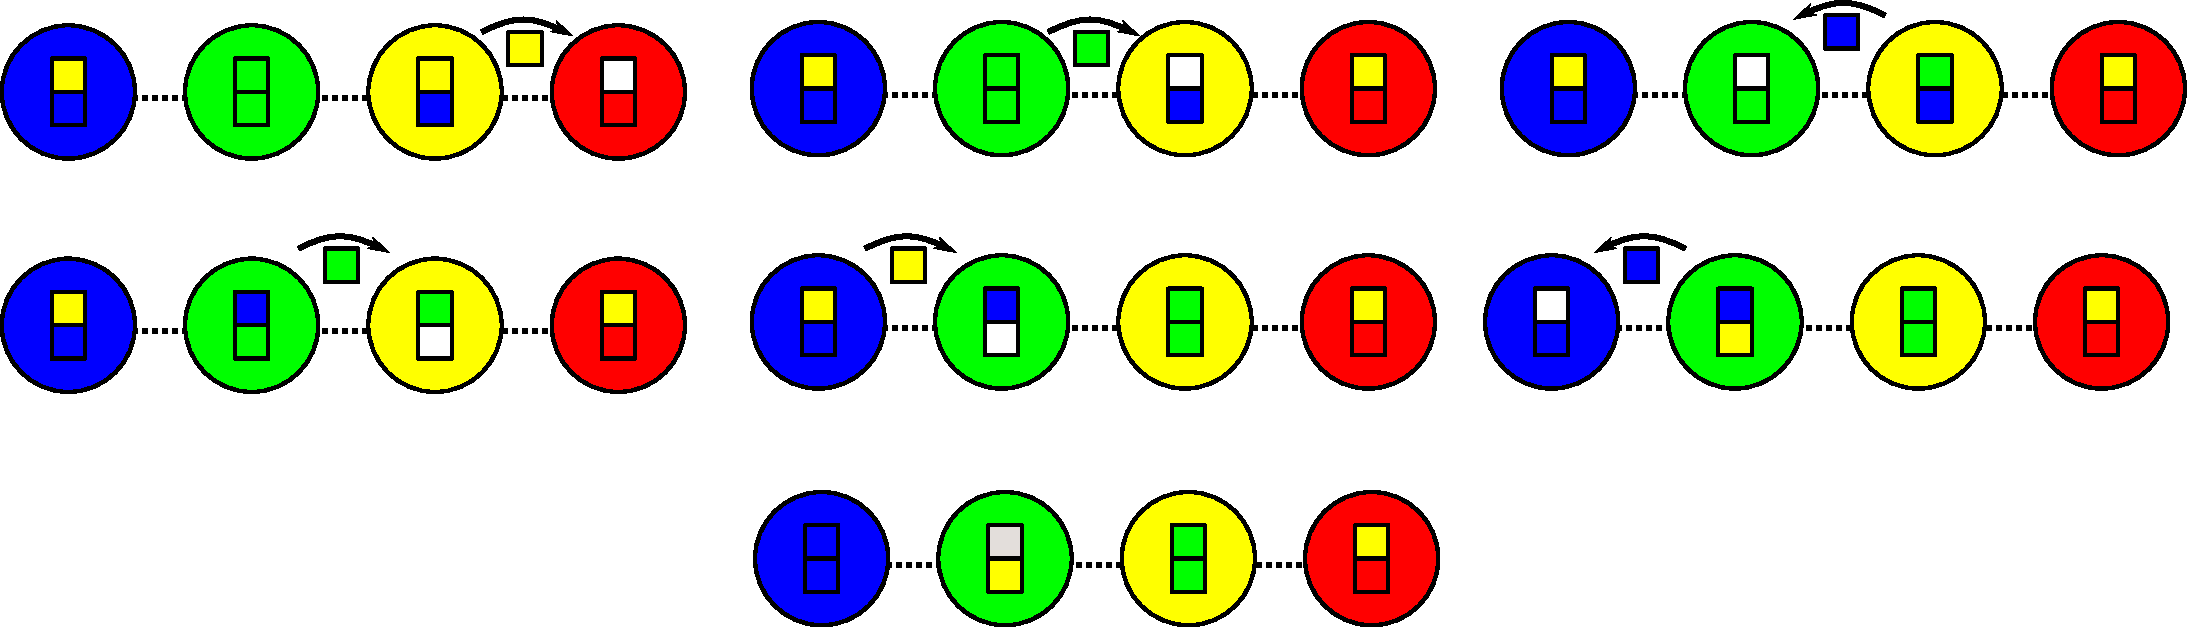
\includegraphics[width=0.8\linewidth]{img/baseball_ex3.pdf}
  \end{center}

  \begin{itemize}
  \item On peut maintenant oublier les bonshommes de la première maison, qui sont à leur place définitive.
  \item On recommence de la même manière avec la deuxième maison, et ainsi de suite ...
  \end{itemize}
\end{frame}

\begin{frame}{Ce qu'il faut retenir du base-ball multicolore: corrections d'algorithmes}
  Cet algorithme n'est pas tellement plus complexe ou plus long que le
  précédent, mais il est correct, lui.

  \begin{block}{Comment être sûr de la \alert{correction} de cet algorithme?}
    \begin{itemize}
    \item \structure{On pourrait tester tous les cas}. Ici, il n'y a pas de limite au nombre de maisons - il est donc impossible de vérifier tous les cas, tout comme il est impossible de compter jusqu'à l'infini. Cependant, on peut se contenter d'une preuve partielle en se limitant à tester tous les cas succeptibles d'être rencontrés - par exemple jusqu'à 20 ou 50 maisons.
    \item \structure{On pourrait écrire une preuve mathématique}. Ce n'est pas trivial, mais les chercheurs en informatique en ont écrite des plus difficiles.
    \item \structure{Cela ressemble vraiment à un algorithme classique} (même
      si cela ne prouve rien, au fond).
    \end{itemize}
  \end{block}

  \begin{block}{Qu'est ce qu'un \alert{algorithme classique}?}
    \begin{itemize}
    \item Les informaticiens apprennent par cœur des algorithmes (abstraits) à l'école.
    \item Face à un problème nouveau, on cherche à se raccrocher à des problèmes connus.
      \begin{itemize}
      \item On se raccroche en trouvant des analogies ou en décomposant en plusieurs problèmes connus.
      \item Par exemple, quand des collègues informaticiens jouent au crêpier, ils demandent avant tout si c'est "une tour de Hanoï".
      \end{itemize}
    \item Ici, notre algorithme est proche d'un "tri à bulle", autre algorithme bien connu. Mais cette ressemblance ne suffit pas à prouver la correction de notre algorithme. Pour la prouver, on pourrait démontrer que notre algorithme est un cas particulier du tri à bulle.
    \end{itemize}
  \end{block}

  \begin{block}{Les algorithmes de tri sont ultra classiques en informatique}
    \begin{itemize}
    \item Ils sont assez simple pour expliquer les grandes lignes aux élèves\\
      (comme «diviser pour régner» et autres grandes idées similaires -- récursivité, algorithmes gloutons, \ldots)
    \item Les ordinateurs trient très souvent des données, car beaucoup de problèmes sont plus simples après\\
      (trouver un livre donné est plus simple dans une bibliothèque rangée, par exemple)
    %\item Du coup, au chapitre 2 de mon cours d'algorithmique, on apprend 5
      %algorithmes de tri par cœur: Tri à bulle, tri par sélection, tri par
      %insertion, tri fusion, tri rapide (et quinze autres en exos).
    \item \alert{Les musiciens font leurs gammes, les informaticiens débutants
      apprennent leurs algorithmes}
    \end{itemize}
  \end{block}

  \begin{block}{Que font les chercheurs en informatique?}
    \begin{itemize}
    \item Certains d'entre eux améliorent les algorithmes connus, ou en
      inventent de nouveaux
    \item Il faut également démontrer la correction de ces algorithmes
    \item Quand plusieurs algorithmes existent, on étudie leurs \alert{performances} respectives
    \item (d'autres chercheurs améliorent matériel et logiciel, établissent des
      modèles, etc)
    \end{itemize}
  \end{block}
\end{frame}

\begin{frame}{Ce qu'il faut retenir du base-ball multicolore: performance d'algorithmes}
  \begin{block}{Comment comparer la performance des algorithmes?}
    \begin{itemize}
    \item Simplement en comptant les étapes. Par exemple sur le crépier, placer la grande crêpe prend au pire 3 coups - et c'est pareil pour les crêpes suivantes. Donc, dans le pire des cas notre algorithme prendra $3\times n$ coups pour trier la pile.
    \item La performance de mon algo dépend beaucoup de la situation initiale:
      \begin{itemize}
      \item Si c'est déjà trié, c'est de la chance, je n'ai rien à faire
        (\alert{meilleur cas}).
      \item Si j'ai vraiment pas de bol, je dois faire les 3 étapes pour chaque crêpe (\alert{pire cas}).
      \item En pratique, j'ai souvent une situation initiale intermédiaire (\alert{cas moyen}).
      \end{itemize}

      Il faut bien comprendre que ceci ne dépend pas vraiment de l'algorithme, mais plutôt de la situation initiale. Le pire cas n'est pas un bug de l'algorithme, mais une situation initiale qui n'aide pas vraiment notre façon de faire (pour estimer la performance d'un cas moyen, il faut utiliser des probabilités).
    \item En pratique, une estimation de la performance est suffisante. Savoir
      qu'un algorithme nécessite environ $n^2$ étapes suffit, inutile de préciser que c'est $n^2+4$ ou $n^2-2$, ou même $5\times n^2$ - pour des grandes valeurs de $n$ c'est sensiblement la même chose\ldots On note cette estimation de la complexité $O(n^2)$.
    \end{itemize}
  \end{block}

  \begin{block}{À la recherche du meilleur algorithme possible}
    \begin{itemize}
    \item On arrive parfois à montrer qu'on a le meilleur algorithme possible. Par exemple on ne peut pas trier les éléments en moins de $n$ étapes, car on doit forcément tous les considérer.
    \item On peut aussi prouver qu'un tri comparatif ne peut pas se faire en moins de $n\times log(n)$ étapes, car il n'accumule pas assez d'information pour choisir la bonne permutation en moins d'étapes.
    \item Mais la plupart du temps, on ne sait pas prouver que l'algorithme connu est le meilleur possible. C'est alors le meilleur \textit{connu}, sans être forcément le meilleur \textit{possible}.
    \end{itemize}
  \end{block}

  \begin{block}{À la recherche de problèmes difficiles}
    \begin{itemize}
    \item On peut classifier les problèmes en fonction de la performance des algorithmes les résolvant. \\
      (cela permet de se forger un sens commun de ce qui est faisable avec un ordinateur et éviter les problèmes si difficiles qu'ils sont quasi impossibles)
    \item Il existe énormément de problèmes relativement simples pour lesquels personne ne connaît de bon algorithme, sans que personne n'arrive non plus à démontrer qu'un tel algorithme n'existe pas.
    \item L'activité suivante sera l'occasion d'explorer un peu cette classification des problèmes très durs.
    \end{itemize}
  \end{block}
\end{frame}

%%% Local Variables: 
%%% mode: latex
%%% TeX-master: "CSIRL"
%%% End: 


\hyphenation{meil-leures}

% récupérer un peu de place au dessus des titres
\renewcommand{\chapterheadstartvskip}{\vspace *{-\baselineskip }} 

\newenvironment{encart}[2]
{
  \begin{center}
  \vbox{
  \colorbox{light-blue}{
  \begin{minipage}{\linewidth}
  \begin{center}\textbf{#1}\end{center}
  \end{minipage}}\\
  \colorbox{light-gray}{
  \begin{minipage}{\linewidth}
  #2
  \end{minipage}}
  }
  \end{center}
}

\title{Les Algorithmes} 
\date{}
%\author{author}


\AtBeginDocument{
  \def\labelitemi{$\bullet$}
  \def\labelitemii{$\bullet$}
  \def\labelitemiii{$\bullet$}
}

%\boldmath

\definecolor{light-gray}{gray}{0.95}
\definecolor{light-blue}{rgb}{0.7 0.7 0.9}

\begin{document}

%%%
%%% Couverture et ours
%%%

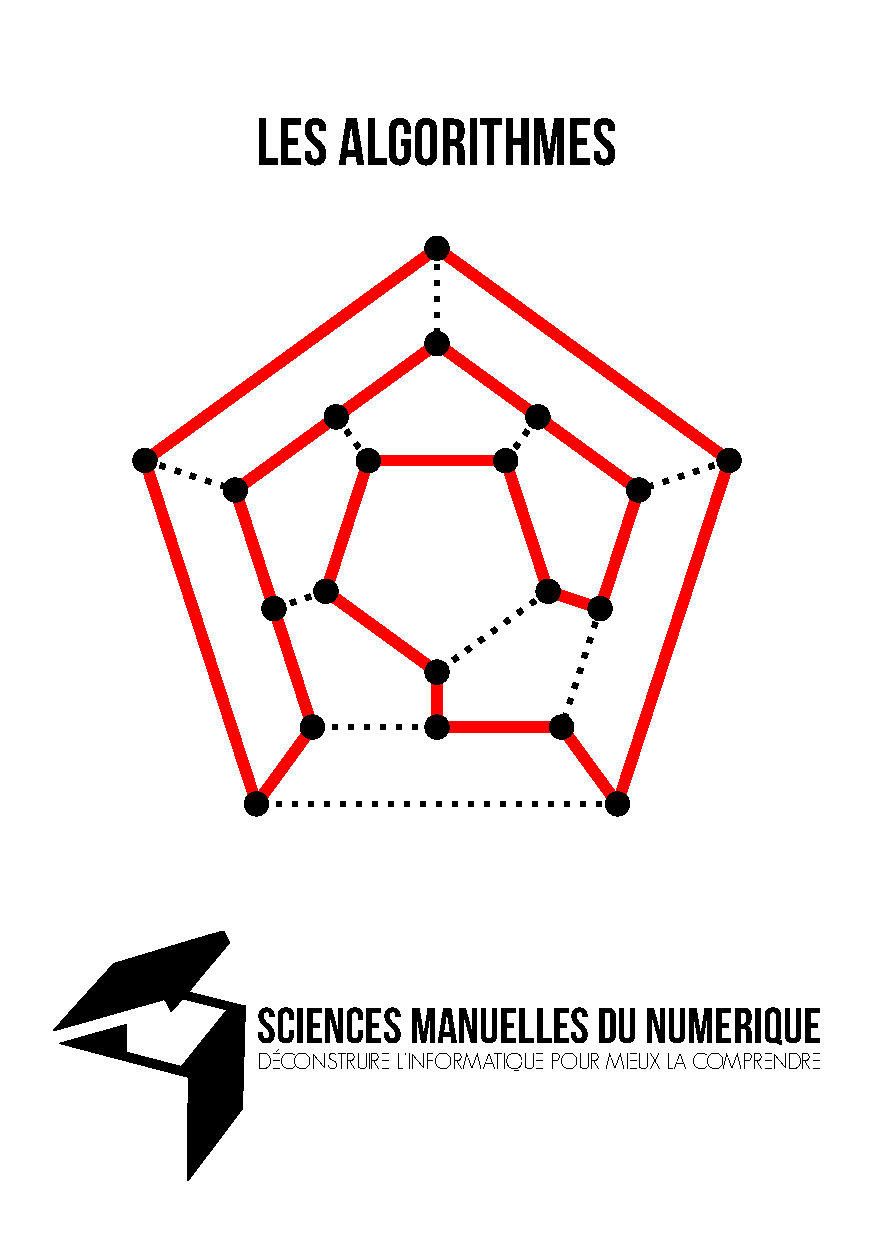
\includepdf[pages=1]{img/couverture.pdf}

\copyright\ 2011-2013 membres du projet SMN. Tous droits réservés.
  
"Sciences Manuelles du Numérique" est un \textbf{projet libre et ouvert}: vous
pouvez copier et modifier librement les ressources de ce projet sous les
conditions données par la CC-BY-SA (en bref, vous pouvez diffuser et modifier
ces ressources à condition que vous donniez les mêmes droits aux utilisateurs de
vos copies).

\bigskip

Ce projet est porté par l'association \textbf{Nancy Bidouille}
(\url{http://www.nybi.cc}), avec le soutien d'\textbf{Inria}
(\url{http://www.inria.fr}).
  
\bigskip

\begin{itemize}
\item Page web : \url{http://www.loria.fr/~quinson/Mediation/CSIRL/}
\item Sources et ressources : \url{http://github.com/jcb/CSIRL}
\item Pour nous joindre : \url{discussions@listes.nybi.cc}
\end{itemize}

\bigskip
~\hfill
\includegraphics[width=0.3\textwidth]{img/logo_nybicc.pdf}\hfill

\includegraphics[width=0.3\textwidth]{img/logo_inria.pdf}\hfill~

\vfill
\textbf{Crédits image}

{\footnotesize

P1: Chemin hamiltonien par Ch. Sommer (licence GFDL/CC-BY-SA)\\
\url{http://en.wikipedia.org/wiki/File:Hamiltonian_path.svg}

P\pageref{img:CSmajor}: Computer Science Major (licence CC-BY-NC)\\
\url{http://abstrusegoose.com/206}

% P\pageref{img:realprog}: Real programmers: \alert{Dessin non libre, à refaire.}
% \url{http://www.ninisworld.com/oddsends/justforfun/50realprogrammers.html}

%P\pageref{img:tsp}: exemple de TSP adapté de Wikipedia (licence GFDL/CC-BY-SA)\\
%\url{http://en.wikipedia.org/wiki/File:Aco_TSP.svg}
P\pageref{img:electric:city}: Electric City par Mathias M, licence CC-BY-SA
\url{http://www.flickr.com/photos/mathias_m/342535332/}
  
P\pageref{img:tsp_xkcd}: Travelling Salesman Problem par XKCD (licence CC BY-NC 2.5)\\
\url{http://xkcd.com/399/}
}

%%%
%%% Début des hostilités
%%%


% \chapter*{Computer Science IRL\footnote{\textit{Computer Science} signifie
% science informatique en anglais, tandis que \textit{IRL} est l'abréviation
% utilisée sur internet pour décrire la vraie vie, ce qui n'est pas sur
% internet.} -- Informatique sans ordinateur}
\chapter*{La science informatique, sans ordinateur}

% Contrairement à ce que beaucoup de monde pense, les ordinateurs ne sont pas la
% seule raison d'être de l'informatique. Pour preuve, ce projet développe
% diverses activités à faire avec des pions, des jetons ou des bouts de bois,
% mais sans aucun ordinateur et même sans électricité. Pourtant, ces petits jeux
% permettront à chacun de découvrir de manière ludique les notions au cœur de
% l'informatique: ce qu'est un algorithme et qu'est ce qui fait qu'un algorithme
% est meilleur qu'un autre, ou encore comment coder et transmettre une
% information.

Trop souvent, lorsque l'on parle d'informatique, on pense à l'ordinateur utilisé
comme outil. L'informatique devient alors l'art d'utiliser l'ordinateur pour une
tâche donnée, ou de le réparer. Pourtant, dans les entrailles de cette machine
se cache un domaine scientifique très vaste, dont les ramifications dépassent
largement l'ordinateur et son fonctionnement.

Avec le projet \textbf{Sciences Manuelles du Numérique}, nous vous proposons
d'explorer la science informatique{\ldots} en retirant l'ordinateur ! Pour cela,
nous avons conçu une série d'activités ludiques introduisant des notions
fondamentales de l'informatique par le biais d'un support matériel, pour
\textit{apprendre avec les mains}. Ces activités sont regroupées en séances
thématiques, permettant ainsi d'aborder les notions fondamentales de manière
cohérente et progressive.

%\begin{block}{Introduction: les principales caractéristiques d'un ordinateur}
    %\begin{itemize}
    %\item \structure{Il est très \alert{rapide}:} il peut calculer de 1 à 1
    %  million en moins d'une seconde
    %\item \structure{Il est parfaitement \alert{obéissant}:} il fait
    %tout le temps exactement ce qu'on lui demande
    %\item \structure{Il est absolument \alert{stupide}:} il exécute les
      %ordres qu'on lui donne, sans la moindre capacité d'initiative.
      %\begin{itemize}
      %\item Par exemple, si on demande à un ordinateur de s'arrêter, il le fait{\ldots}
      %\item Autre exemple, quand j'indique à des amis comment venir chez moi,
        %je leur donne des indications comme ``troisième à droite'' ou ``à gauche
        %au 2ieme feu''. Si je me trompe dans mes indications (``à gauche'' au lieu
        %de ``à droite'') et que cela les ferait prendre l'autoroute à
        %contre-sens, mes amis vont faire preuve de sens commun et ne pas
        %appliquer la consigne. Les ordinateurs n'ont \textbf{aucun} sens commun.
        % \item Bug (n.m.): consigne erronée donnée par un humain et appliquée
        %   bêtement par une machine.
      %\end{itemize}
    %\end{itemize}
  %\end{block}\vspace{-.5\baselineskip}

\section*{La séance algorithmique}

L'objectif de cette séance est d'introduire la notion fondamentale
d'\textbf{al\-gorithme}. Qu'est-ce-que c'est ? A quoi ça sert ? Comment sont-ils
inventés ? Pour cette séance, comptez \textbf{une heure et demi à deux
  heures}. Bien entendu, il ne s'agit pas d'un cours complet sur le sujet ! Si
vous souhaitez aller plus loin, voici un cours en 48h :
\url{http://www.loria.fr/~quinson/Teaching/TOP/}.

Les animateurs d'ateliers trouveront des conseils et astuces à la fin de chaque
activité dans \og le coin de l'animateur \fg ; mais les conseils les plus
importants sont certainement les suivants :

\begin{itemize}
\item appropriez-vous les activités. Pratiquez-les à l'avance et n'hésitez pas à
  ne pas suivre les consignes à la lettre;
\item ces activités sont des bases de discussion avec les participants, il n'y a
  pas d'évaluation à la fin;
\item évitez les introductions théoriques; commencez par les activités, elles
  serviront de support pour discuter de la théorie.
\end{itemize}

\begin{center}
  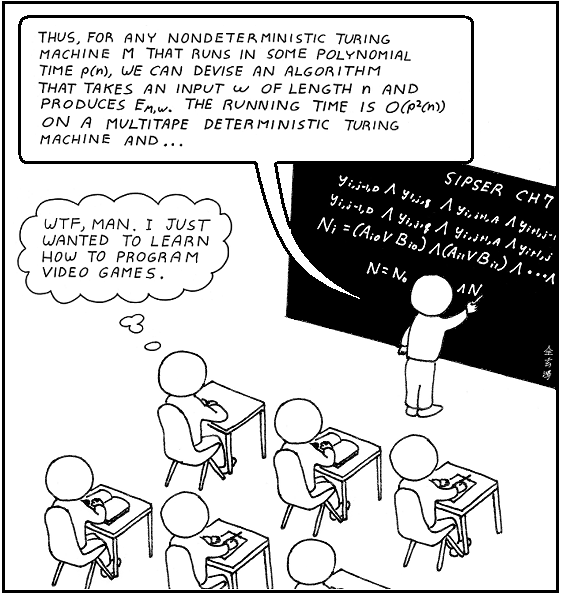
\includegraphics[width=0.7\linewidth]{img/computer_science_major.PNG}
  \label{img:CSmajor}
\end{center}

\begin{frame}{Activité: le jeu de Nim}

  Voici un premier petit jeu simple, pour rentrer dans le sujet.

  \begin{block}{Matériel}
    \begin{itemize}
    \item 16 petits objets (clous, allumettes, boulettes de papier ... peu importe !)
    \end{itemize}
  \end{block}

  \begin{block}{Règle du jeu}
    \begin{itemize}
    \item Disposer les 16 objets sur une table
    \item Les deux joueurs prennent tour à tour 1, 2 ou 3 objets
    \item Le joueur qui prend le dernier objet à gagné
    \end{itemize}
  \end{block}

  \bigskip \bigskip  \bigskip \bigskip

  \begin{center}
    % rendre l'illustration plus utile en la transformant en exemple de partie?
    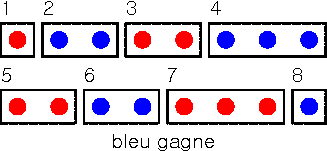
\includegraphics[width=0.8\linewidth]{img/nim.pdf}
  \end{center}

\end{frame}

\begin{frame}{Ce qu'il faut retenir du jeu de Nim}

  \begin{block}{L'intérêt majeur de ce jeu est qu'il est sans suspense 
      {\color{black}\normalsize(voire, sans intérêt ;)}}
    \begin{itemize}
    \item Celui qui commence (\structure{J1}) perd, car il existe un truc pour
      que \structure{J2} gagne à tous les coups
    \item \structure{Stratégie gagnante:} Laisser 4, 8, 12 ou 16 objets à
      l'adversaire (un multiple de 4)
    \end{itemize}
  \end{block}

  \begin{columns}
    \begin{column}{0.7\linewidth}

      \begin{block}{Se convaincre de l'efficacité de la stratégie gagnante}
        Prenons le dernier tour comme exemple. Il reste 4 objets, et J1 joue.

        \begin{itemize}
        \item Si J1 prend \alert{1} objet, J2 en prend \structure{3} (dont le dernier) 
        \item Si J1 prend \alert{2} objets, J2 en prend \structure{2} (dont le dernier)
        \item Si J1 prend \alert{3} objets, J2 en prend \structure{1} (le dernier) 
        \end{itemize}        
        %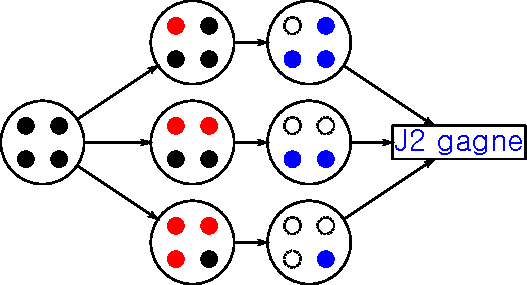
\includegraphics[width=0.6\linewidth]{img/nim4.pdf}

        Dans ce cas, si J2 sait jouer, J1 perd à tous les coups.  En appliquant la même méthode, J2 peut guider le jeu de manière à passer de 16 objets à 12, puis 8 et enfin 4. Donc, si J2 sait jouer, J1 a perdu la partie avant même de commencer.
        
        \center{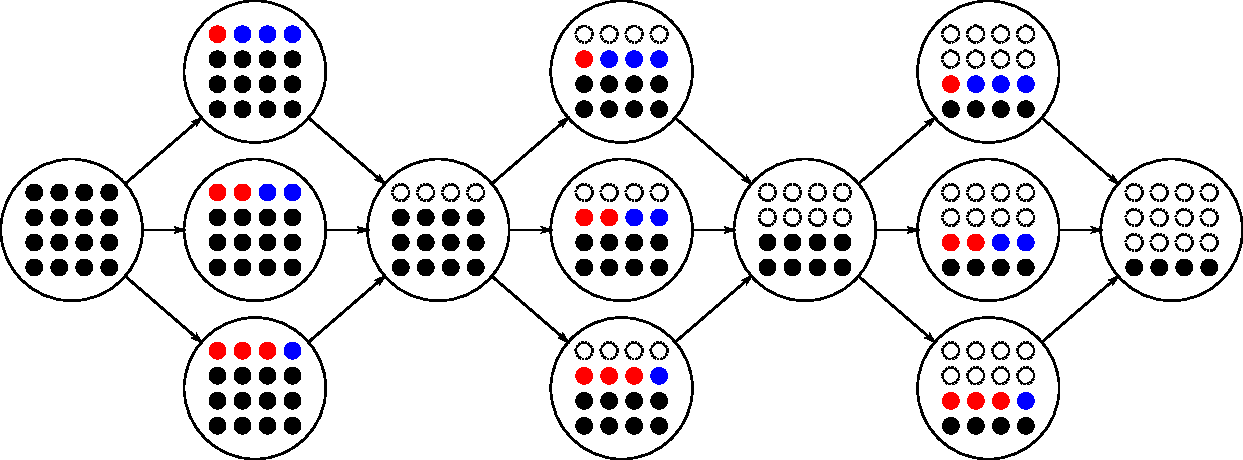
\includegraphics[width=\linewidth]{img/nim16.pdf}}
      \end{block}

    \end{column}
    \begin{column}{0.3\linewidth}

      \begin{block}{Pour aller plus loin}
        On pourrait imaginer un cas plus général du jeu de Nim :

        \begin{itemize}
          \item Il y a $N$ objets sur la table au début du jeu (pour notre version, $N=16$)
          \item Un joueur peut prendre jusqu'à $X$ objets à la fois (pour notre version, $X=3$)
        \end{itemize}

        Quelles modifications doit-on apporter à notre stratégie gagnante pour qu'elle marche dans le cas général ?
      \end{block}

    \end{column}
  \end{columns}

  \begin{block}{Le rapport avec l'informatique}
    \begin{itemize}
    \item Passer de la situation initiale à la situation finale à coup sûr demande d'avoir
      une \textit{stratégie gagnante}
    \item C'est un \alert{\textbf{algorithme}} en informatique, une recette de
      cuisine ou un manuel de montage de meubles
    \item Pour se faire obéir du tas de fils, l'informaticien cherche
      l'algorithme pour résoudre le problème,\\
      puis il écrit le \alert{\textbf{programme}} (traduction de l'algorithme
      dans un langage informatique)
    \end{itemize}
  \end{block}

\end{frame}

\begin{frame}{Activité: Le crêpier psycho-rigide}

  \begin{block}{Matériel}
    \begin{itemize}
    \item des planchettes en bois de tailles et de couleurs différentes (faces reconnaissables)
    \item éventuellement une pelle à tarte pour retourner les planchettes
    \end{itemize}
  \end{block}

  \begin{block}{Règle du jeu}
    \begin{itemize}
      \item \structure{Installation :} Faire une pile désordonnée de crêpes.
      \item \structure{Objectif :} ranger les crêpes de la plus grande (en bas) à la plus petite (au haut), face colorée vers le haut.
      \item \structure{Coup autorisé :} prendre une ou plusieurs crêpes sur le haut de la pile, et de les reposer à l'envers.
    \end{itemize}
  \end{block}

  \bigskip \bigskip \bigskip

  \begin{center}
    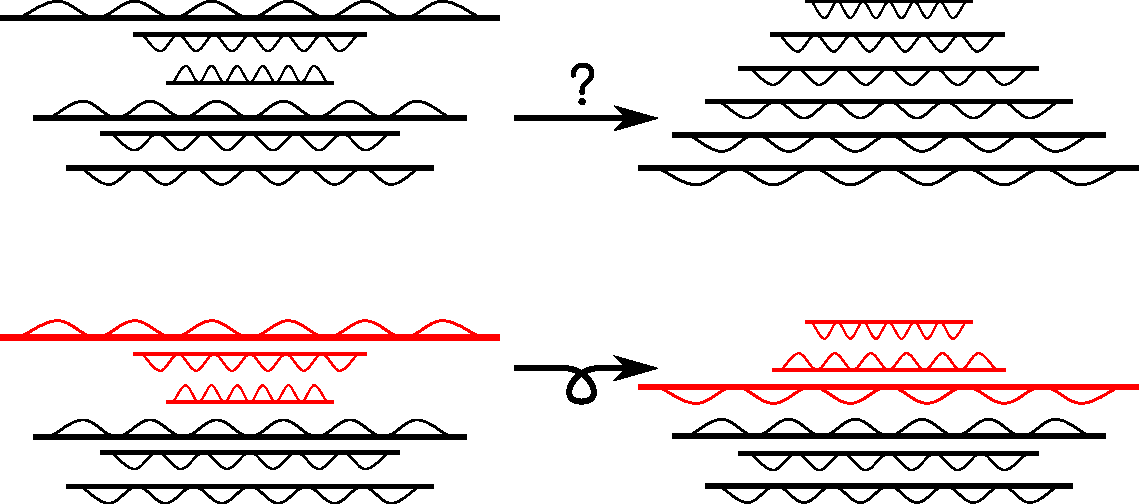
\includegraphics[width=0.8\linewidth]{img/crepier.pdf}
  \end{center}

\end{frame}

\begin{frame}{Ce qu'il faut retenir du  crêpier psycho-rigide}

  \begin{columns}
    \begin{column}{.7\linewidth}
      \begin{block}{Un algorithme}
        \begin{itemize}
        \item n'a d'intérêt que si on peut l'expliquer
        \item doit être suffisamment simple pour pouvoir l'expliquer à une machine
        \item \alert{\textbf{«Diviser pour mieux régner»}} : on essaie toujours de décomposer un algorithme en tâches simples
        \end{itemize}
      \end{block}

      \begin{block}{L'algorithme que doit suivre le crêpier est :}
        \begin{itemize}
        \item ramener la plus grande crêpe en haut de la pile
        \item retourner pour que la face brûlée soit vers le haut
        \item retourner la pile de sorte à mettre la plus grande crêpe en bas
        \item réitérer avec la crêpe de taille inférieure
        \end{itemize}
      \end{block}

      \begin{block}{Le rapport avec l'informatique}
        \begin{itemize}
        \item l'informaticien passe son temps à trouver des algorithmes et  à les expliquer à la machine
        \item le principe \alert{\textbf{«Diviser pour mieux régner»}} est fondamental en informatique
        \end{itemize}
      \end{block}
    \end{column}

    \begin{column}{.3\linewidth}
      \begin{block}{Pour aller plus loin}
        Selon l'état initial de la pile de crêpes, le nombre minimum de coups nécessaires pour la ranger varie.

        \begin{itemize}
          \item Quel est le meilleur état initial possible (qui demandera le moins de coups pour ranger) ?
          \item Quel est le pire état initial possible ?
          \item Combien faut-il de coups pour ranger une pile de $N$ crêpes dans le pire des cas ?
        \end{itemize}
      \end{block}
    \end{column}
  \end{columns}
      
\end{frame}

\begin{frame}{Ce qu'il faut retenir du crêpier psycho-rigide : performance d'algorithmes}

  \begin{block}{Pourquoi évaluer la performance d'un algorithme ?}

    Évaluer la performance d'un algorithme nous permet :

    \begin{itemize}
      \item de se faire une idée du temps nécessaire pour résoudre un problème de plus grande taille (combien de temps pour un million de crêpes ?) ;
      \item de le comparer à d'autres aglorithmes résolvant le même problème, pour savoir lequel est le meilleur.
    \end{itemize}

  \end{block}

  \begin{block}{Comment évaluer la performance d'un algorithme ?}

    \begin{itemize}
      \item On compte le nombre de coups nécessaires dans le cas général. Pour le crêpier :
        \begin{itemize}
          \item pour ranger une crêpe, il faut entre $0$ coups (la crêpe est déjà rangée) et $3$ coups (amener en haut, retourner, amener à sa place) ;
          \item pour $n$ crêpes (cas général), il faut entre $0$ et $3 \times n$ coups ;
          \item la performance d'un algorithme sur un cas particulier dépend donc beaucoup de l'état initial, mais en règle générale on s'intéresse surtout aux cas intermédiaires, qui sont les plus probables.
        \end{itemize}
      \item $n$ est une variable qui exprime la taille du problème. La performance d'un algorithme est notée comme une fonction de la taille du problème nommée $O$.
      \item La performance exprime un ordre de grandeur plutôt qu'une évaluation précise du temps d'exécution. Pour des grandes valeurs de $n$, il n'est pas très utile de faire la distinction entre $O(n)$, $O(n+4)$ ou encore $O(3 \times n)$ - surtout quand on compare avec un autre algorithme dont la performance est $O(n^2)$. 
      \item On simplifie donc en retirant les constantes pour ne garder que les termes les plus importants. Pour le crêpier, on notera la performance de notre algorithme $O(n)$ ; on dit alors que le temps de calcul croit \textit{linéairement} avec $n$. En revanche, un algorithme $O(n^2)$ aurait une croissance \textit{quadratique}, et un algorithme $O(2^n)$ aurait une croissance \textit{exponentielle}.
     \end{itemize}
  \end{block}

  \begin{block}{À la recherche du meilleur algorithme possible}
    \begin{itemize}
    \item On arrive parfois à montrer qu'on a le meilleur algorithme possible. Par exemple on ne peut pas trier les éléments en moins de $n$ étapes, car on doit forcément tous les considérer.
    \item On peut aussi prouver qu'un tri comparatif ne peut pas se faire en moins de $n\times log(n)$ étapes, car il n'accumule pas assez d'information pour choisir la bonne permutation en moins d'étapes.
    \item Mais la plupart du temps, on ne sait pas prouver que l'algorithme connu est le meilleur possible. C'est alors le meilleur \textit{connu}, sans être forcément le meilleur \textit{possible}.
    \end{itemize}
  \end{block}

  %\begin{block}{À la recherche de problèmes difficiles}
    %\begin{itemize}
    %\item On peut classifier les problèmes en fonction de la performance des algorithmes les résolvant. \\
      %(cela permet de se forger un sens commun de ce qui est faisable avec un ordinateur et éviter les problèmes si difficiles qu'ils sont quasi impossibles)
    %\item Il existe énormément de problèmes relativement simples pour lesquels personne ne connaît de bon algorithme, sans que personne n'arrive non plus à démontrer qu'un tel algorithme n'existe pas.
    %\item L'activité suivante sera l'occasion d'explorer un peu cette classification des problèmes très durs.
    %\end{itemize}
  %\end{block}
\end{frame}

%\newcommand{\maisonPair}[5]{ \begin{tikzpicture}
  \node[name=m,shape=regular polygon,regular polygon sides=#3,minimum size=22mm,rotate=(360/#3)]{};
  \node[name=b,shape=regular polygon,regular polygon sides=#4,minimum size=14mm,rotate=(360/#4)/2]{};
  \foreach \base/\maison in {#5} {
    \draw[shift=(m.corner \base)]
       node[shape=ellipse,fill=\maison,draw=black,rotate=((360/#3)*(\base-1))+(360/#3/2)] {~~};
  }
  \foreach \bb in {1,...,#4} {
    \draw[shift=(b.corner \bb)] node[name=bb \bb]{};
  }
  \foreach \base/\maison in {#1} {
    \draw[shift=(b.corner \base)]
       node[name=bb \base,shape=circle,fill=\maison,draw=black,inner sep=.1]
       {~~~};
%         {\footnotesize\base};
  }
  #2
\end{tikzpicture} }
\newcommand{\maisonImpair}[5]{ \begin{tikzpicture}
  \node[name=m,shape=regular polygon,regular polygon sides=#3,
        minimum size=22mm, inner sep=0pt]{};
  \node[name=b,shape=regular polygon,regular polygon sides=#4,minimum size=14mm]{};
  \foreach \base/\maison in {#5} {
    \draw[shift=(m.corner \base)]
       node[shape=ellipse,fill=\maison,draw=black,rotate=(360/#3)*(\base-1)] {~~};
  }
  \foreach \base/\maison in {#1} {
    \draw[shift=(b.corner \base)]
       node[shape=circle,fill=\maison,draw=black,inner sep=.1] {~~~};
  }
  \foreach \bb in {1,...,#4} {\draw[shift=(b.corner \bb)] node[name=bb \bb] {};}
%  \foreach \bb in {1,...,#4} {\draw[shift=(b.corner \bb)] node[name=bb \bb]{\tiny\bb};}%debug the bonshommes names
  #2
\end{tikzpicture} }

\newcommand{\maisonQuatre}[2]{\maisonPair{#1}{#2}{4}{12}{1/A,2/B,3/C,4/D}}
\newcommand{\maisonCinq}[2]{\maisonImpair{#1}{#2}{5}{20}{1/A,2/B,3/C,4/D,5/E}}
\newcommand{\maisonSix}[2]{\maisonPair{#1}{#2}{6}{24}{1/A,2/B,3/C,4/D,5/E,6/F}}
\newcommand{\maisonSept}[2]{\maisonImpair{#1}{#2}{7}{28}{1/A,2/B,3/C,4/D,5/E,6/F,7/G}}

\colorlet{A}{green!60}
\colorlet{B}{red!80}
\colorlet{C}{purple!40}
\colorlet{D}{black!2!yellow}
\colorlet{E}{blue!70}
\colorlet{F}{orange!80}
\colorlet{G}{olive}
\colorlet{H}{magenta}
\colorlet{I}{lime}
\colorlet{J}{pink}

\newcommand{\pawn}[1]{\tikz \draw node[shape=circle,fill=#1,draw=black,inner sep=.1] {~~~};}



%%%%%%%%%%%%%%%%%%%%%%%%%%%%%%%%%%%%%%%%%%%%%%%%%%%%%%%%%%%%%%%%%%%%%%%%%%%%%%%%%%%%%%%
\begin{frame}{Activité: Base-ball multicolore}
  \begin{block}{Matériel nécessaire}
    \begin{itemize}
    \item Plusieurs équipes bien différentiables, chacune composée d'une maison et de deux bonshommes (des legos, des bouts de bois, des cailloux, du fil électrique de différentes couleurs, ou autres) 
    \item 4 équipes au minimum. On peut mettre des équipes supplémentaires pour augmenter la difficulté.
    \end{itemize}
  \end{block}

  \begin{block}{Règles du jeu (exemple à quatre équipes)}
    \begin{itemize}
      \item \structure{Installation :} disposer 4 maisons autour du terrain et répartir 7 bonshommes au hasard sur les maisons (le bonhomme restant n'est pas utilisé).
      \item \structure{Coup autorisé :} déplacer un seul bonhomme à la fois, vers la maison contenant un seul bonhomme, depuis une des deux maisons voisines (interdit de traverser le terrain).
    \item  \structure{Objectif :} Ramener tous les bonshommes dans la maison de leur couleur.
    \end{itemize}
  \end{block}

  \bigskip

  \begin{columns}
    \begin{column}{0.27\linewidth}
    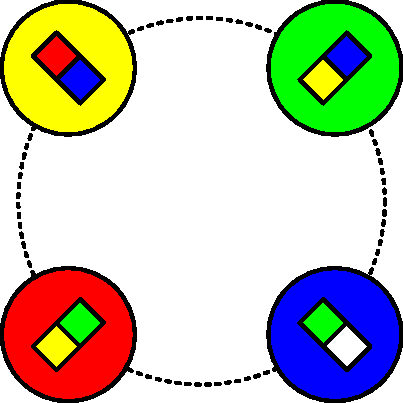
\includegraphics[width=\linewidth]{img/baseball_init.pdf}\\
    \center{État initial}
    \end{column}
    \begin{column}{0.27\linewidth}
    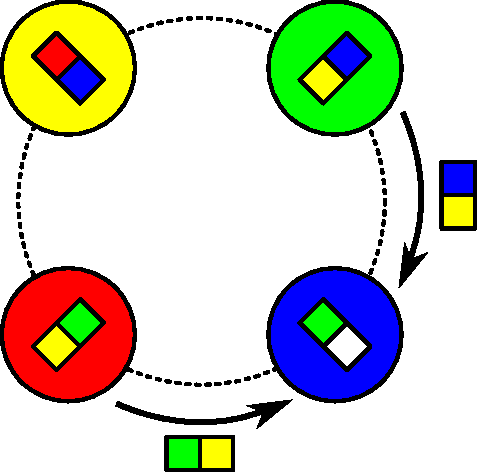
\includegraphics[width=\linewidth]{img/baseball_coup.pdf}\\
    \center{Coup autorisé}
    \end{column}
    \begin{column}{0.27\linewidth}
    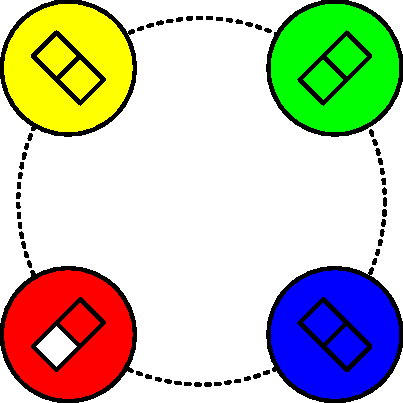
\includegraphics[width=\linewidth]{img/baseball_final.pdf}\\
    \center{État final}
    \end{column}
  \end{columns}

  \bigskip
  \begin{block}{Objectif de l'activité}
    Le plus important dans cet exercice n'est pas tant de résoudre le problème que d'\structure{expliquer clairement} comment on fait. On cherche donc l'\alert{algorithme} permettant de résoudre le problème.
  \end{block}
\end{frame}
%%%%%%%%%%%%%%%%%%%%%%%%%%%%%%%%%%%%%%%%%%%%%%%%%%%%%%%%%%%%%%%%%%%%%%%%%%%%%%%%%%%%%%%%%
%\newcommand{\flecherond}[1]{
  %\draw[ultra thick] (0,0) circle (3mm);
  %\draw[ultra thick,rotate=#1*72] (3mm,0) -- +(-.15,-.08);
  %\draw[ultra thick,rotate=#1*72] (3mm,0) -- +(.08,-.15);
  %\draw[fill=white,draw=white,rotate=#1*72] (3mm,2.5pt) circle (2pt);
%}
\begin{frame}{Un premier algorithme pour le base-ball multicolore}
  En suivant les règles du jeu, on observe que quelque soit la disposition des bonshommes, il existe toujours 4 coups possibles : déplacer vers la case vide un des 4 bonshommes présents dans les deux maisons voisines.

  Notre algorithme sera donc une méthode permettant de choisir à chaque étape quel coup jouer parmis les 4 possibles.

  \begin{block}{L'algorithme}
    \begin{itemize}
    \item On ne s'autorise à tourner que dans un seul sens. Ainsi, le nombre de coups possibles descends de 4 à 2 (car 2 bonshommes tourneraient à l'envers).
    \item Parmis les 2 coups restants, on déplace le bonhomme qui a la plus grande distance à parcourir avant d'arriver à sa maison (Si la distance est la même, c'est que les deux bonhommes ont la même couleur - les deux coups sont donc équivalents).
    \end{itemize}
  \end{block}

  \begin{block}{Exemple d'exécution}
    \begin{center}
      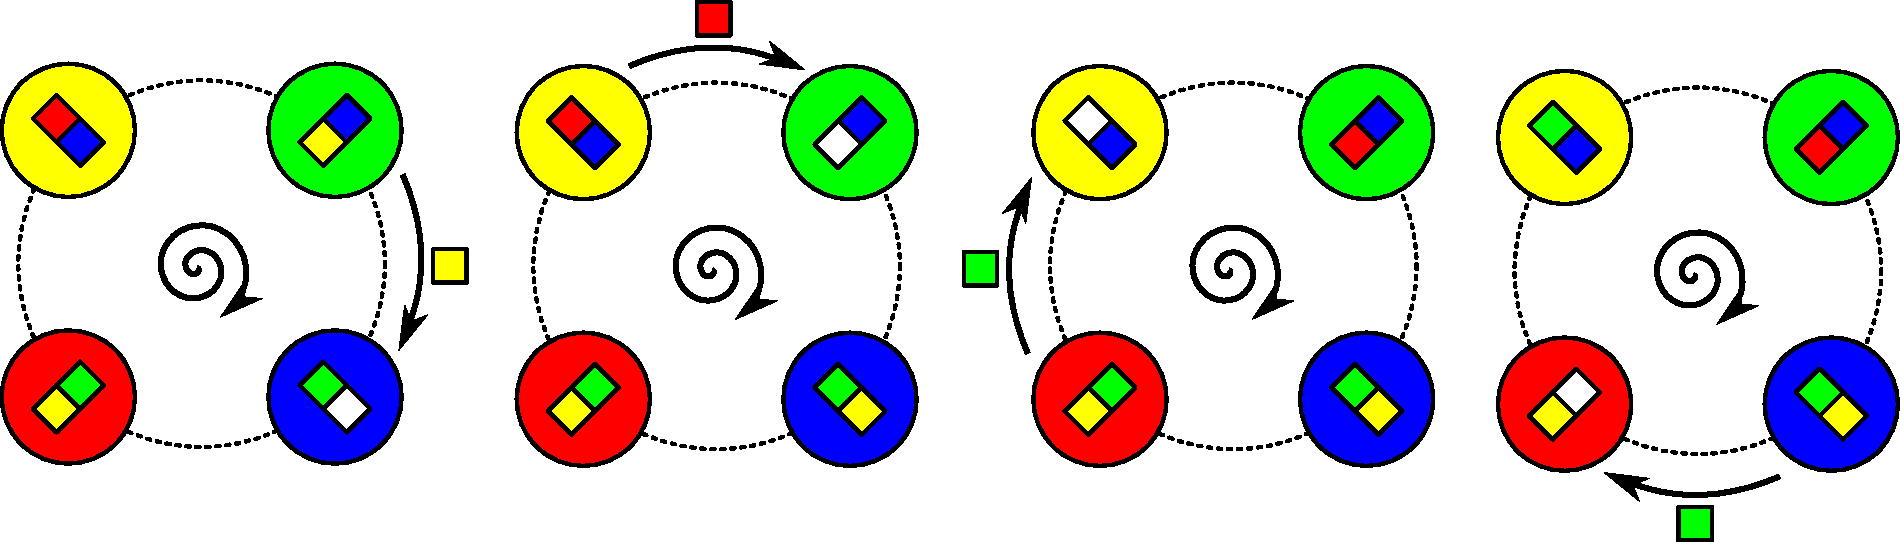
\includegraphics[width=\linewidth]{img/baseball_ex1.pdf}
    \end{center}

  Ici, nous n'avons représenté que les 4 premières étapes. mais l'algorithme arrive à la solution en 15 étapes.
  \end{block}
\end{frame}

\begin{frame}{Étude du premier algorithme pour le base-ball multicolore}
  \begin{block}{Cet algorithme semble attirant}
    \begin{itemize}
    \item Il est très simple: on pourrait l'expliquer à un ordinateur
    \item Il est relativement rapide: 15 coups pour 7 bonshommes, ce n'est pas si mal
    \item Seul problème: cet algorithme est faux: dans certains cas, il ne termine jamais\ldots
    \end{itemize}
  \end{block}

  \begin{block}{Exemple d'exécution incorrecte}
    Il suffit de partir d'une situation gagnée et d'inverser deux bonshommes pour mettre notre algorithme en échec.
\end{block}
  \begin{center}
    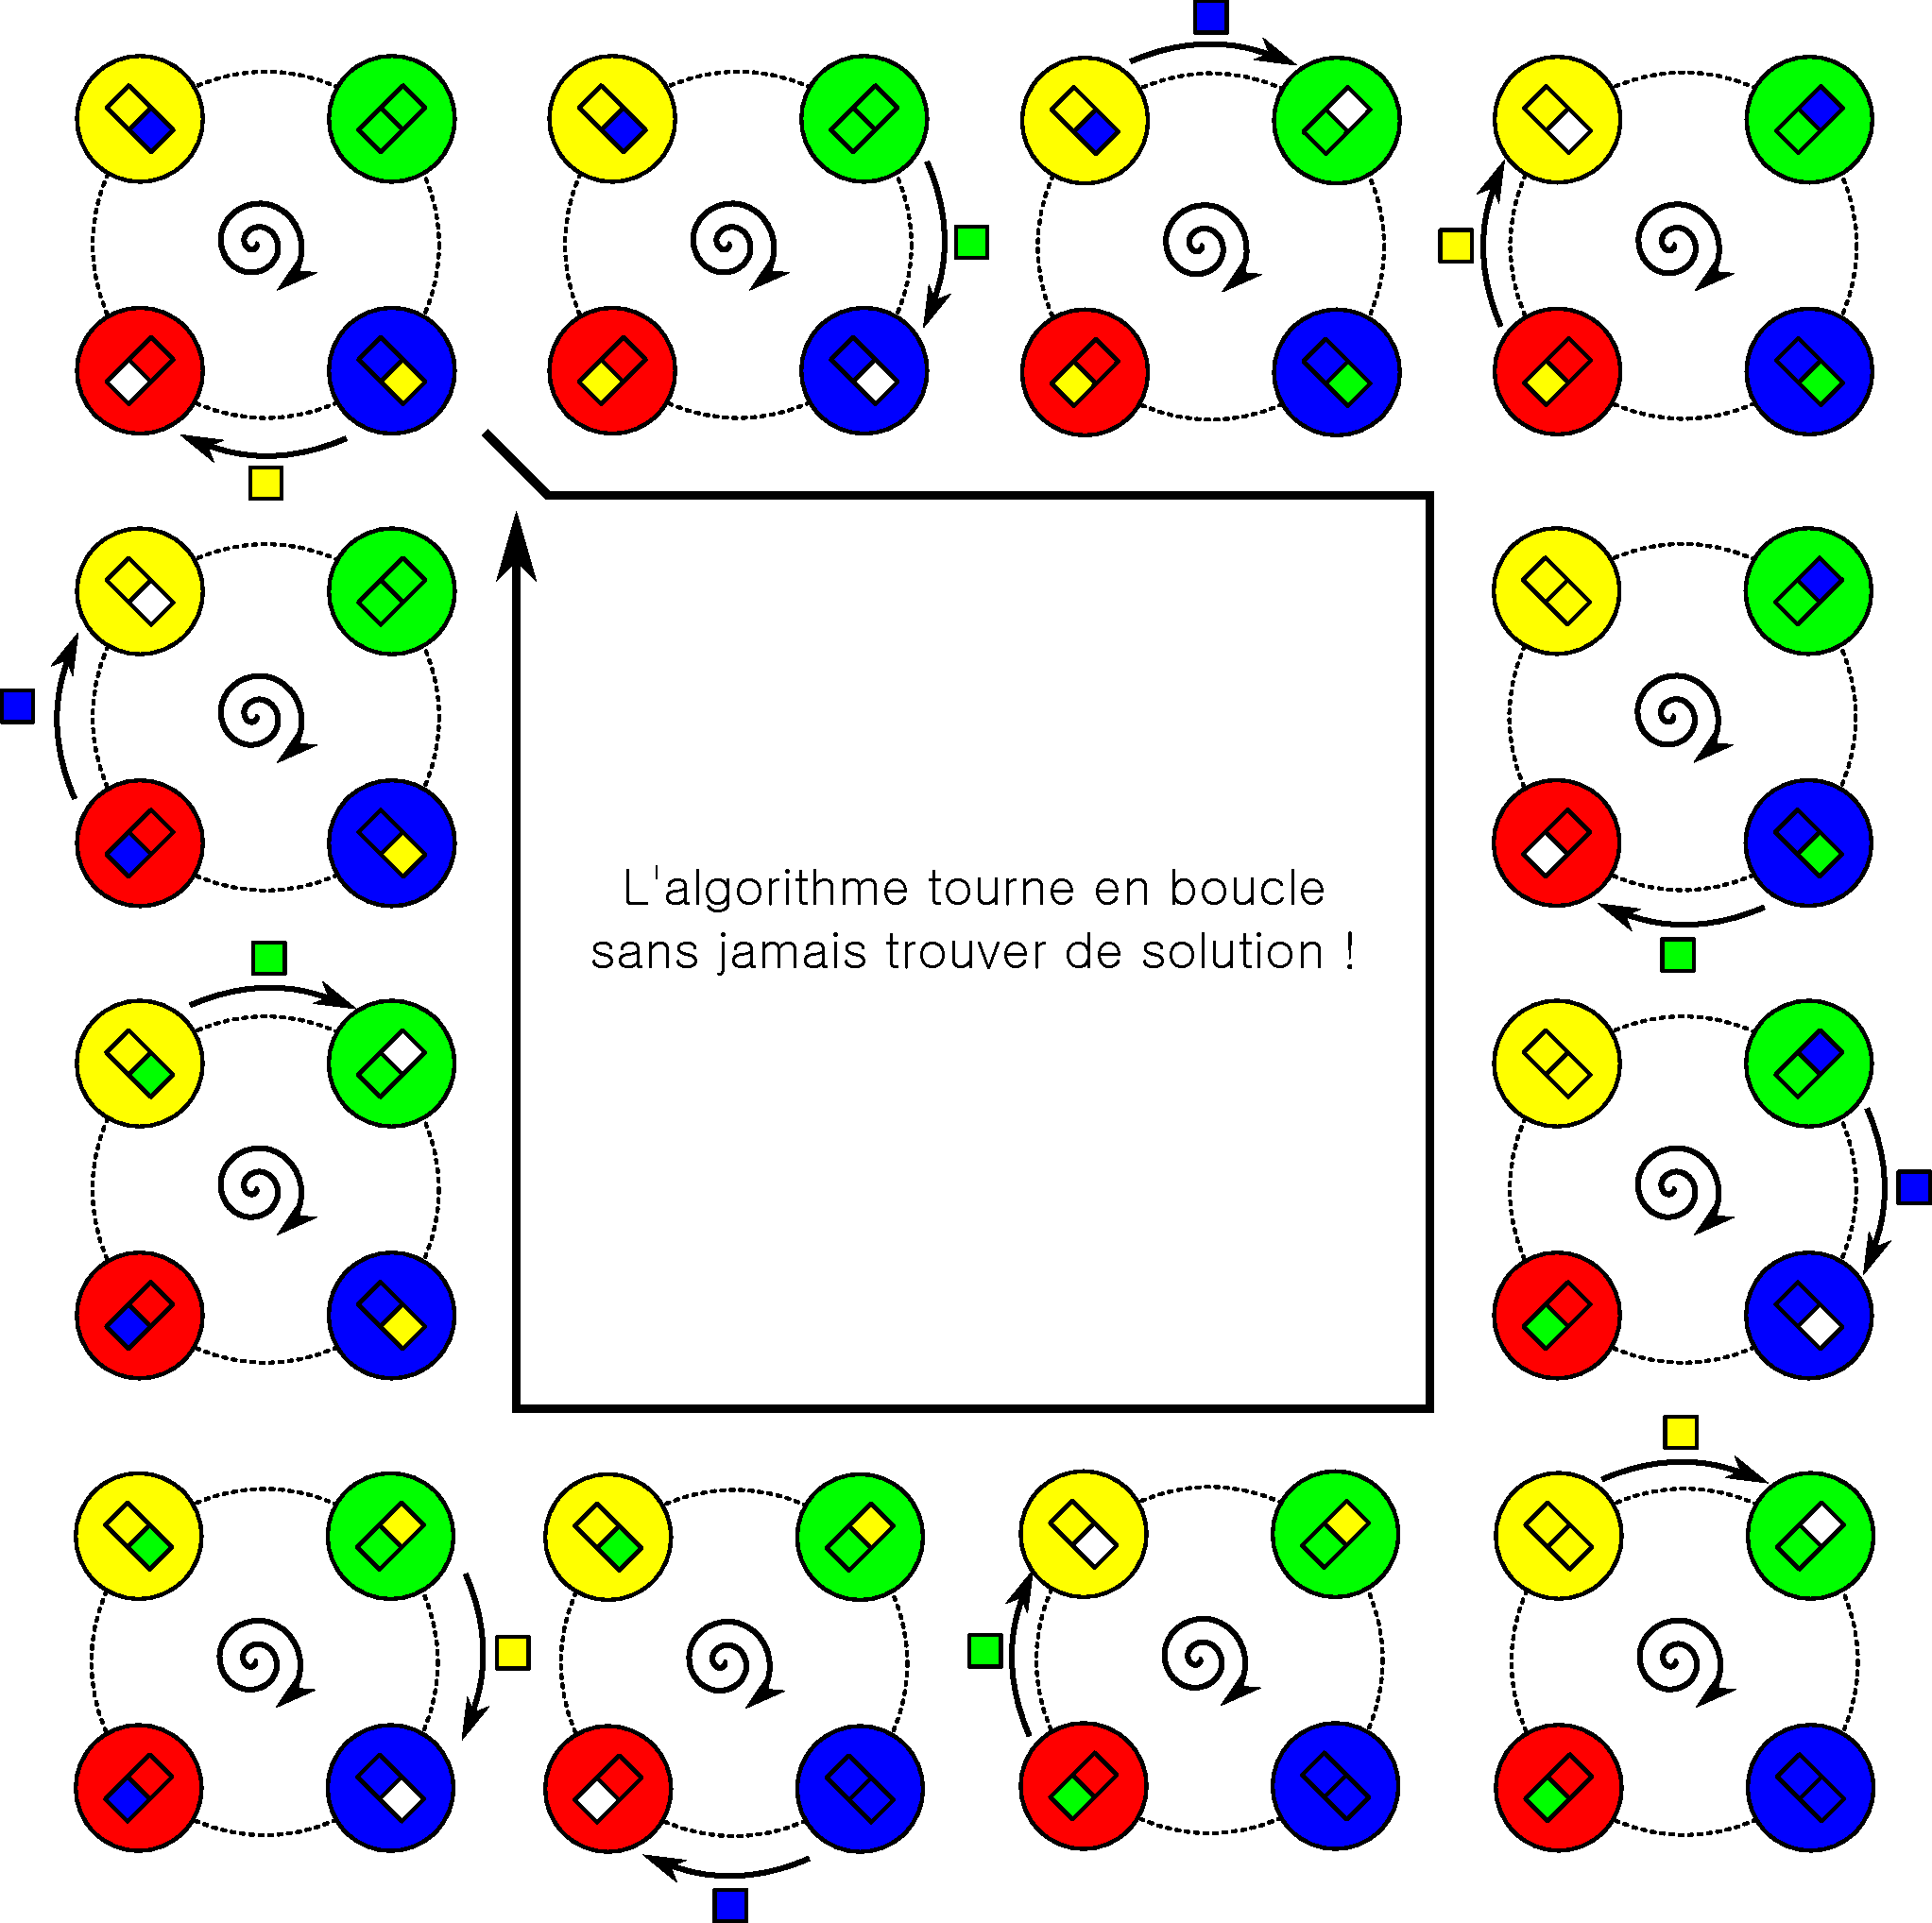
\includegraphics[width=0.8\linewidth]{img/baseball_ex2.pdf}
  \end{center}
\end{frame}

%%%%%%%%%%%%%%%%%%%%%%%%%%%%%%%%%%%%%%%%%%%%%%%%%%%%%%%%%%%%%%%%%%%%%%%%%%%%%%%%%%%%%%%%
\begin{frame}{Un autre algorithme pour le base-ball multicolore}
  \begin{block}{Apprendre de ses échecs: {\color{black}notre algorithme boucle parfois à l'infini}}
    \begin{itemize}
    \item Pour réparer cela, le plus simple est de s'interdire de boucler, en
      coupant le cercle.
    \item Pour ne pas se tromper, le plus simple est de placer les maisons en ligne.
    \end{itemize}

    \begin{center}
      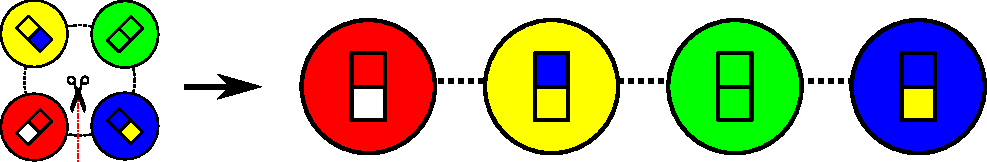
\includegraphics[width=0.8\linewidth]{img/baseball_ligne.pdf}
    \end{center}
  \end{block}

  \bigskip

  \begin{block}{Apprendre de ses réussites: {\color{black}le crépier}}
    \begin{itemize}
    \item On a cherché à réduire la taille du problème à peu à peu\\
      {(il y a 7 crèpes à trier. La plus grande va définitivement à sa place; il
        reste 6 crèpes à trier)}
    \item On s'est fixé des objectifs intermédiaires, qui décomposent le
      problème en étapes que je sais faire\\
      {(mettre la plus grande en haut pour parvenir à la mettre en bas)}
    \end{itemize}
  \end{block}

  \begin{block}{Nouvel algorithme}
    \begin{itemize}
    \item On s'occupe d'abord des bonshommes de la première maison, et on n'y touche plus ensuite.
    \item On répète pour la deuxième maison, et ainsi de suite pour toutes les autres.
    \item Pour ammener les bonhommes dans leur maison, on déplace tous ceux qui gènent.
    \item Pour déplacer ceux qui gènent, on déplace le trou pour leur faire de la place.
    \end{itemize}
  \end{block}

  \begin{center}
    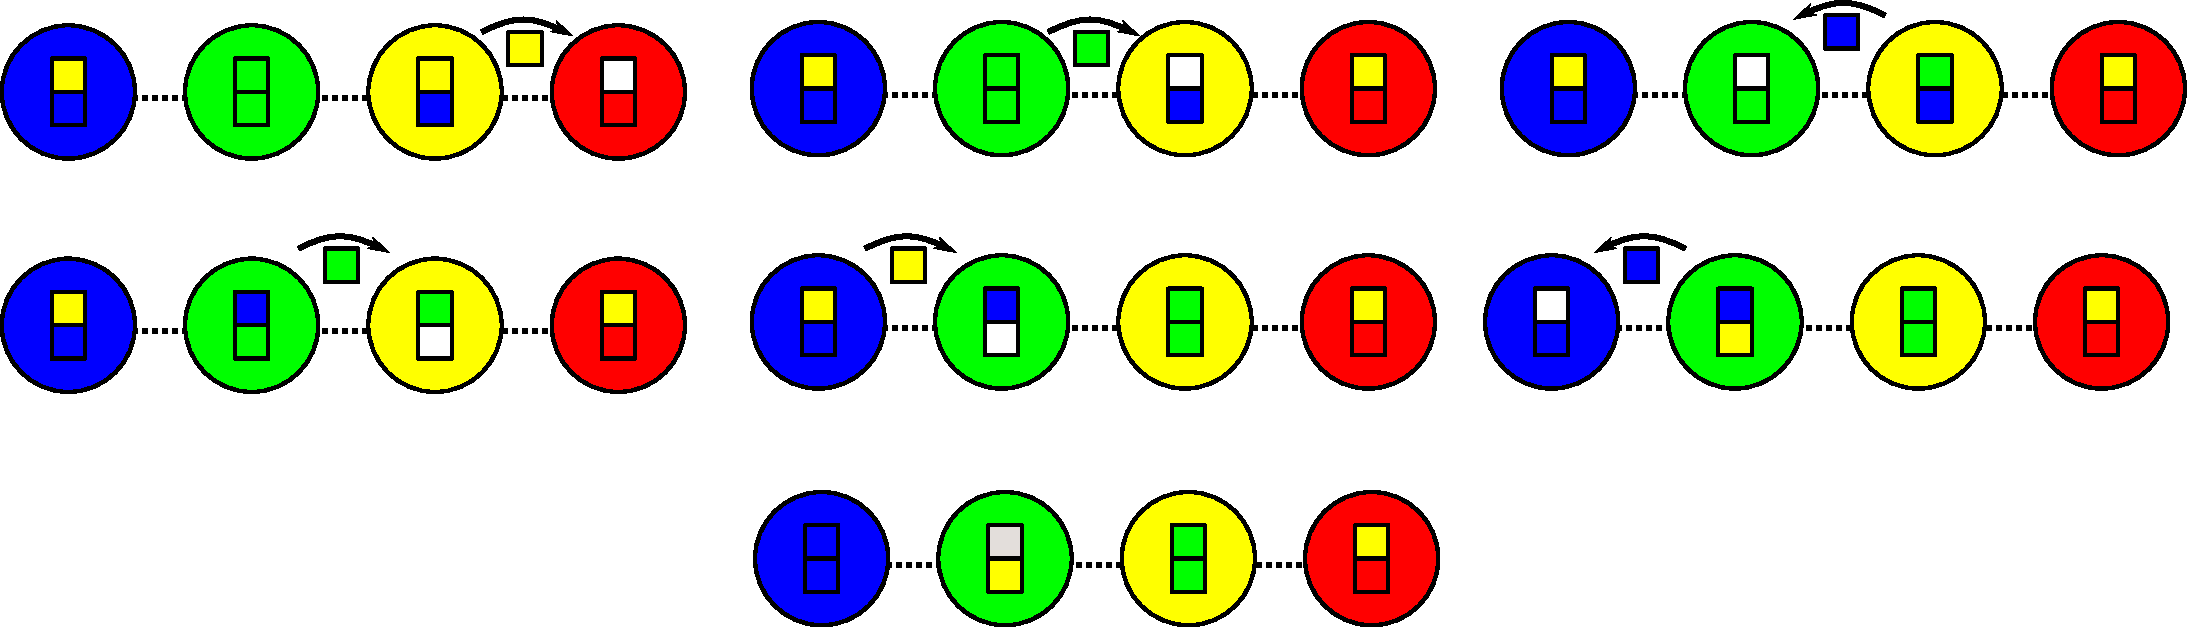
\includegraphics[width=0.8\linewidth]{img/baseball_ex3.pdf}
  \end{center}

  \begin{itemize}
  \item On peut maintenant oublier les bonshommes de la première maison, qui sont à leur place définitive.
  \item On recommence de la même manière avec la deuxième maison, et ainsi de suite ...
  \end{itemize}
\end{frame}

\begin{frame}{Ce qu'il faut retenir du base-ball multicolore: corrections d'algorithmes}
  Cet algorithme n'est pas tellement plus complexe ou plus long que le
  précédent, mais il est correct, lui.

  \begin{block}{Comment être sûr de la \alert{correction} de cet algorithme?}
    \begin{itemize}
    \item \structure{On pourrait tester tous les cas}. Ici, il n'y a pas de limite au nombre de maisons - il est donc impossible de vérifier tous les cas, tout comme il est impossible de compter jusqu'à l'infini. Cependant, on peut se contenter d'une preuve partielle en se limitant à tester tous les cas succeptibles d'être rencontrés - par exemple jusqu'à 20 ou 50 maisons.
    \item \structure{On pourrait écrire une preuve mathématique}. Ce n'est pas trivial, mais les chercheurs en informatique en ont écrite des plus difficiles.
    \item \structure{Cela ressemble vraiment à un algorithme classique} (même
      si cela ne prouve rien, au fond).
    \end{itemize}
  \end{block}

  \begin{block}{Qu'est ce qu'un \alert{algorithme classique}?}
    \begin{itemize}
    \item Les informaticiens apprennent par cœur des algorithmes (abstraits) à l'école.
    \item Face à un problème nouveau, on cherche à se raccrocher à des problèmes connus.
      \begin{itemize}
      \item On se raccroche en trouvant des analogies ou en décomposant en plusieurs problèmes connus.
      \item Par exemple, quand des collègues informaticiens jouent au crêpier, ils demandent avant tout si c'est "une tour de Hanoï".
      \end{itemize}
    \item Ici, notre algorithme est proche d'un "tri à bulle", autre algorithme bien connu. Mais cette ressemblance ne suffit pas à prouver la correction de notre algorithme. Pour la prouver, on pourrait démontrer que notre algorithme est un cas particulier du tri à bulle.
    \end{itemize}
  \end{block}

  \begin{block}{Les algorithmes de tri sont ultra classiques en informatique}
    \begin{itemize}
    \item Ils sont assez simple pour expliquer les grandes lignes aux élèves\\
      (comme «diviser pour régner» et autres grandes idées similaires -- récursivité, algorithmes gloutons, \ldots)
    \item Les ordinateurs trient très souvent des données, car beaucoup de problèmes sont plus simples après\\
      (trouver un livre donné est plus simple dans une bibliothèque rangée, par exemple)
    %\item Du coup, au chapitre 2 de mon cours d'algorithmique, on apprend 5
      %algorithmes de tri par cœur: Tri à bulle, tri par sélection, tri par
      %insertion, tri fusion, tri rapide (et quinze autres en exos).
    \item \alert{Les musiciens font leurs gammes, les informaticiens débutants
      apprennent leurs algorithmes}
    \end{itemize}
  \end{block}

  \begin{block}{Que font les chercheurs en informatique?}
    \begin{itemize}
    \item Certains d'entre eux améliorent les algorithmes connus, ou en
      inventent de nouveaux
    \item Il faut également démontrer la correction de ces algorithmes
    \item Quand plusieurs algorithmes existent, on étudie leurs \alert{performances} respectives
    \item (d'autres chercheurs améliorent matériel et logiciel, établissent des
      modèles, etc)
    \end{itemize}
  \end{block}
\end{frame}

\begin{frame}{Ce qu'il faut retenir du base-ball multicolore: performance d'algorithmes}
  \begin{block}{Comment comparer la performance des algorithmes?}
    \begin{itemize}
    \item Simplement en comptant les étapes. Par exemple sur le crépier, placer la grande crêpe prend au pire 3 coups - et c'est pareil pour les crêpes suivantes. Donc, dans le pire des cas notre algorithme prendra $3\times n$ coups pour trier la pile.
    \item La performance de mon algo dépend beaucoup de la situation initiale:
      \begin{itemize}
      \item Si c'est déjà trié, c'est de la chance, je n'ai rien à faire
        (\alert{meilleur cas}).
      \item Si j'ai vraiment pas de bol, je dois faire les 3 étapes pour chaque crêpe (\alert{pire cas}).
      \item En pratique, j'ai souvent une situation initiale intermédiaire (\alert{cas moyen}).
      \end{itemize}

      Il faut bien comprendre que ceci ne dépend pas vraiment de l'algorithme, mais plutôt de la situation initiale. Le pire cas n'est pas un bug de l'algorithme, mais une situation initiale qui n'aide pas vraiment notre façon de faire (pour estimer la performance d'un cas moyen, il faut utiliser des probabilités).
    \item En pratique, une estimation de la performance est suffisante. Savoir
      qu'un algorithme nécessite environ $n^2$ étapes suffit, inutile de préciser que c'est $n^2+4$ ou $n^2-2$, ou même $5\times n^2$ - pour des grandes valeurs de $n$ c'est sensiblement la même chose\ldots On note cette estimation de la complexité $O(n^2)$.
    \end{itemize}
  \end{block}

  \begin{block}{À la recherche du meilleur algorithme possible}
    \begin{itemize}
    \item On arrive parfois à montrer qu'on a le meilleur algorithme possible. Par exemple on ne peut pas trier les éléments en moins de $n$ étapes, car on doit forcément tous les considérer.
    \item On peut aussi prouver qu'un tri comparatif ne peut pas se faire en moins de $n\times log(n)$ étapes, car il n'accumule pas assez d'information pour choisir la bonne permutation en moins d'étapes.
    \item Mais la plupart du temps, on ne sait pas prouver que l'algorithme connu est le meilleur possible. C'est alors le meilleur \textit{connu}, sans être forcément le meilleur \textit{possible}.
    \end{itemize}
  \end{block}

  \begin{block}{À la recherche de problèmes difficiles}
    \begin{itemize}
    \item On peut classifier les problèmes en fonction de la performance des algorithmes les résolvant. \\
      (cela permet de se forger un sens commun de ce qui est faisable avec un ordinateur et éviter les problèmes si difficiles qu'ils sont quasi impossibles)
    \item Il existe énormément de problèmes relativement simples pour lesquels personne ne connaît de bon algorithme, sans que personne n'arrive non plus à démontrer qu'un tel algorithme n'existe pas.
    \item L'activité suivante sera l'occasion d'explorer un peu cette classification des problèmes très durs.
    \end{itemize}
  \end{block}
\end{frame}

%%% Local Variables: 
%%% mode: latex
%%% TeX-master: "CSIRL"
%%% End: 

\begin{frame}{Activité: le plus court chemin}
  
  \begin{block}{Matériel nécessaire}
    \begin{itemize}
    \item Une planche avec des trous au hasard,
    \item autant de longs clous que de trous,
    \item une ficelle suffisamment longue et \alert{qui ne soit pas élastique},
    \item un marqueur.
    \end{itemize}
  \end{block}

  \begin{block}{Règles du jeu}
    \begin{itemize}
    \item \structure{Situation initiale :} les clous sont mis dans les trous, leurs têtes dépassent de la planche, et un bout de la ficelle est attachée à un clou.
    \item \structure{Comment jouer :} faire passer la ficelle \alert{une fois et une seule} par \alert{tous les clous} de la planche, puis revenir au point de départ.
    \item  \structure{Objectif :} obtenir le chemin le plus court possible. À chaque fois qu'un record est battu, on fait une marque sur la ficelle pour le mémoriser.
    \end{itemize}
  \end{block}

  \begin{center}
    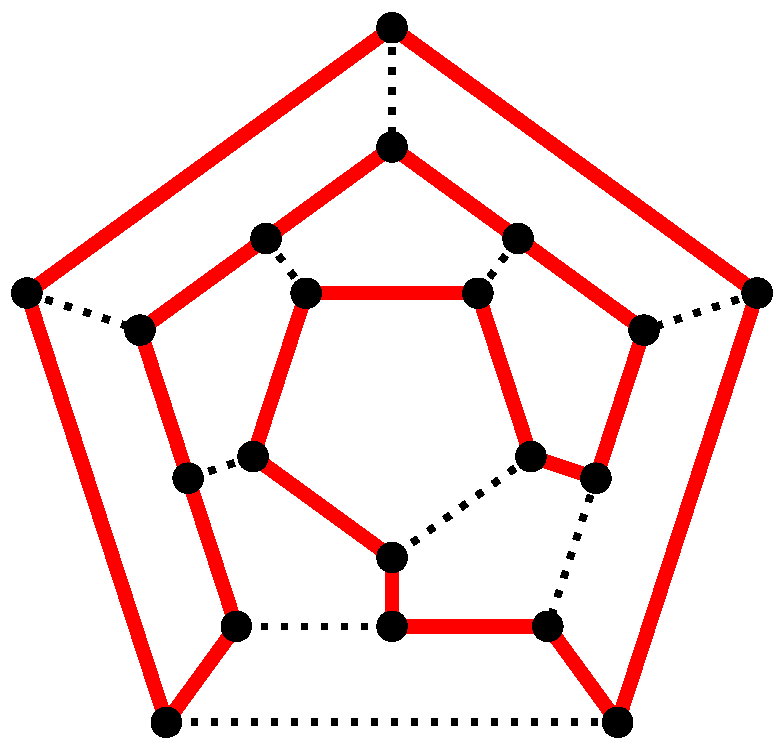
\includegraphics[width=0.3\linewidth]{img/Hamiltonian_path.pdf}
  \end{center}

  \begin{block}{Objectif de l'activité}
    \begin{itemize}
    \item On peut construire un très grand nombre de chemins différents (pour $10$ clous, $10! = 10 \cdot 9 \cdot 8 \cdot \ldots \cdot 2 = 3628800$), et il est très difficile de trouver le meilleur chemin à coup sûr.
    \item A la place, on va chercher des méthodes (algorithmes) pour construire des chemins courts, et comparer leurs résultats.
    \end{itemize}
  \end{block}

\end{frame}

\begin{frame}{Ce qu'il faut retenir du plus court chemin}
  %\centerline{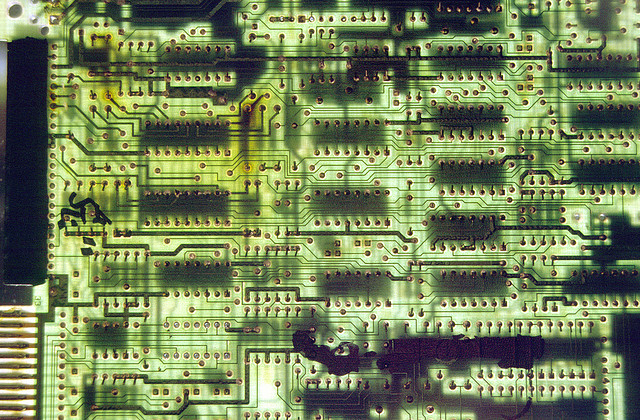
\includegraphics[width=.7\linewidth]{img/electric_city.jpg}\label{img:electric:city}}
  
  \begin{itemize}
    \item Certains problèmes (dont le problème du plus court chemin) sont trop compliqués pour trouver la \alert{solution optimale} en un temps \alert{raisonnable}. Dans de telles situations, on préfère souvent trouver une solution approchée très rapidement, plutôt que de chercher très longtemps la solution optimale. Les méthodes utilisée pour trouver rapidement des solutions approchées sont des \alert{heuristique}.
    \item Le problème du chemin le plus court parait bête mais il fait très difficile, et a de très nombreuses applications dans la vie de tous les jours (comment minimiser la tournée du facteur, la longueur des pistes d'un circuit imprimé, les déplacements d'un bras robotique ...).
  \end{itemize}

  \begin{block}{Trouver la solution optimale}
    
    \begin{itemize}
      \item Dans le cas du chemin le plus court, l'approche naïve consiste à calculer la longueur de tous les chemins et comparer les résultats pour trouver le plus court. La complexité d'une telle approche s'écrit $O(n!)$. Il existe cependant des algorithmes plus efficaces - par exemple, l'algorithme de Held-Karp a une complexité de $O(n^{2}2^n)$. Voici une petite comparaison de l'augmentation de la quantité de calculs nécessaires à mesure que $n$ augmente :

      \bigskip

      \begin{center}
        \begin{tabular}{|l|cccc|}
          \hline
          nombre de sommets       & 5   & 10      & 15            & 20 \\
          \hline
          méthode naïve $O(n!)$   & 120 & 3628800 & 1307674368000 & 2432902008176640000 \\
          Held-Karp $O(n^{2}2^n)$ & 800 & 102400  & 7372800       & 419430400 \\
          \hline
        \end{tabular} 
      \end{center}

      \bigskip

      \item Ce tableau nous montre qu'avec la méthode naïve, en testant un milliard de chemins par seconde, il faudrait plus de \textbf{77 ans} pour trouver le chemin le plus court entre 20 sommets ! En comparaison, l'algorithme Held-Karp met moins d'\textbf{une demi seconde} pour trouver le même résultat !
% les chercheurs classent les problèmes en fonction de la difficulté à trouver des algorithmes efficaces 
    \end{itemize}
  \end{block}

  \begin{center}
    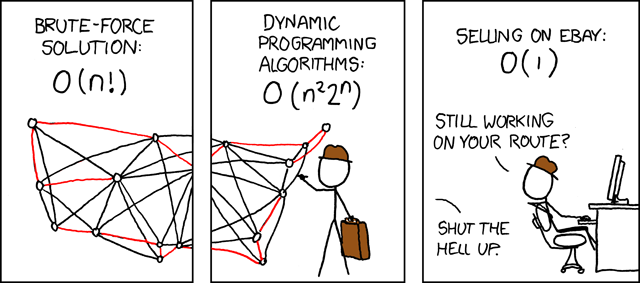
\includegraphics[width=0.8\linewidth]{img/tsp_xkcd.png}
  \end{center}

\end{frame}

\begin{frame}{Ce qu'il faut retenir du plus court chemin}

  \begin{block}{Trouver une solution approchée}


  \end{block}

\end{frame}

    %\item algos NP, NP-difficiles, NP-complets
    %\item C'est un problème qui parait bête mais qui est complexe et qui a de nombreuses applications dans la vie réelle
    %\item Exemple d'application amusante de notion de NP-complétude:  \url{http://arxiv.org/abs/1203.1895}


\end{document}
